% !arara: xelatex:  { action: nonstopmode, synctex: True }
% arara: biblatex
% !arara: makeglossaries
% arara: xelatex: {action: nonstopmode, synctex: True }
% arara: xelatex: {action: nonstopmode, synctex: True }
%%%%%%%%%%%%%%%%%%%%%%%%%%%%%%%%%%%%%%%%%%%%%%%%%%%%%%%%%%%%%%%%%%%%%%%%%%%%
%%%%%%%%%%%%%%%%%%%%%%%%%%%%%%%%%%%%%%%%%%%%%%%%%%%%%%%%%%%%%%%%%%%%%%%%%%%%
%% 
%%   L'encodage de ce fichier doit être UTF-8
%%	 lancer avec Knitr + Xelatex
%%   Liste des choses à faire pour mettre à jour le rapport en nouvelle version
%%   voir issue #1 https://github.com/Eaux-et-Vilaine/passe_bassins/issues/1
%%%%%%%%%%%%%%%%%%%%%%%%%%%%%%%%%%%%%%%%%%%%%%%%%%%%%%%%%%%%%%%%%%%%%%%%%%%%
%%%%%%%%%%%%%%%%%%%%%%%%%%%%%%%%%%%%%%%%%%%%%%%%%%%%%%%%%%%%%%%%%%%%%%%%%%%%
%%%%%%%%%%%%%%%%%%%%%%%%%%%%%%%%%%%%%%%%%%%%%%%%%%%%%%%%%%%%%%%%%%%%%%%%%%%%

%DIV=calc, qui crée une page avec 60 à 70 signes par ligne, dépend bien
%évidemment de la fonte choisie
\documentclass[11pt,twocolumn,titlepage,twoside]{article}\usepackage[]{graphicx}\usepackage[]{color}
% maxwidth is the original width if it is less than linewidth
% otherwise use linewidth (to make sure the graphics do not exceed the margin)
\makeatletter
\def\maxwidth{ %
  \ifdim\Gin@nat@width>\linewidth
    \linewidth
  \else
    \Gin@nat@width
  \fi
}
\makeatother

\definecolor{fgcolor}{rgb}{0.345, 0.345, 0.345}
\newcommand{\hlnum}[1]{\textcolor[rgb]{0.686,0.059,0.569}{#1}}%
\newcommand{\hlstr}[1]{\textcolor[rgb]{0.192,0.494,0.8}{#1}}%
\newcommand{\hlcom}[1]{\textcolor[rgb]{0.678,0.584,0.686}{\textit{#1}}}%
\newcommand{\hlopt}[1]{\textcolor[rgb]{0,0,0}{#1}}%
\newcommand{\hlstd}[1]{\textcolor[rgb]{0.345,0.345,0.345}{#1}}%
\newcommand{\hlkwa}[1]{\textcolor[rgb]{0.161,0.373,0.58}{\textbf{#1}}}%
\newcommand{\hlkwb}[1]{\textcolor[rgb]{0.69,0.353,0.396}{#1}}%
\newcommand{\hlkwc}[1]{\textcolor[rgb]{0.333,0.667,0.333}{#1}}%
\newcommand{\hlkwd}[1]{\textcolor[rgb]{0.737,0.353,0.396}{\textbf{#1}}}%
\let\hlipl\hlkwb

\usepackage{framed}
\makeatletter
\newenvironment{kframe}{%
 \def\at@end@of@kframe{}%
 \ifinner\ifhmode%
  \def\at@end@of@kframe{\end{minipage}}%
  \begin{minipage}{\columnwidth}%
 \fi\fi%
 \def\FrameCommand##1{\hskip\@totalleftmargin \hskip-\fboxsep
 \colorbox{shadecolor}{##1}\hskip-\fboxsep
     % There is no \\@totalrightmargin, so:
     \hskip-\linewidth \hskip-\@totalleftmargin \hskip\columnwidth}%
 \MakeFramed {\advance\hsize-\width
   \@totalleftmargin\z@ \linewidth\hsize
   \@setminipage}}%
 {\par\unskip\endMakeFramed%
 \at@end@of@kframe}
\makeatother

\definecolor{shadecolor}{rgb}{.97, .97, .97}
\definecolor{messagecolor}{rgb}{0, 0, 0}
\definecolor{warningcolor}{rgb}{1, 0, 1}
\definecolor{errorcolor}{rgb}{1, 0, 0}
\newenvironment{knitrout}{}{} % an empty environment to be redefined in TeX

\usepackage{alltt} 
\usepackage{float}
\usepackage[section]{placeins}  %The placeins package provides the command \FloatBarrier
%%============================================================
%%============================================================
%% PACKAGE SETUP

%\SweaveOpts{pdf=TRUE, echo=FALSE, fig=FALSE, eps=FALSE, tidy=T, width=4,
%height=4, keep.source=TRUE}
%% Input and language packages.
\usepackage[UTF8]{inputenc} %encodage du fichier source
\usepackage[T1]{fontenc}  %gestion des accents (pour les pdf) 
\usepackage{aeguill} % guillemets
%\usepackage[english]{babel}
% 'babel/polyglossia' detected but 'csquotes' missing.
\usepackage[french]{babel}
\usepackage{csquotes}
\usepackage{amsmath} %equation
\usepackage{fontspec}
\usepackage{unicode-math}
\usepackage{microtype}
\defaultfontfeatures{Scale=MatchLowercase}
\setmainfont{Segoe UI}[
   Scale = 1.0,
   BoldFont = Segoe UI Semibold ,
   BoldItalicFont = Segoe UI Semibold Italic]
\setmathfont{Segoe UI}
%\setmathfont{Segoe UI Italic}
%\setmathfont{Segoe UI Semibold Italic}
%Selecting fonts locally
% If you want to use a font for a small section of your document it's best to
% define a new font family called with comment \titlefont{...}
\newfontfamily\titlefont{Georgia} 



%% Parskip is the extra vertical space inserted before a paragraph. It has a natural length of zero 
%but should be a rubber length so that it may be stretched in a flushbottom
% environment. To increase \parskip to skip a line between paragraphs one could use \addtolength{\parskip} {\baselineskip}.
\usepackage{parskip}



%% Sets space between lines.
\usepackage{setspace} 


\usepackage{longtable}
\usepackage{booktabs}
%% Using captions in floating environment. Note: might not work with other packages.
%\usepackage{caption}
\usepackage[labelfont={color=orange_EV,bf}]{caption} % pour éviter les problème de
% place entre le header et le tableau et légendes en gras
\addto\captionsfrench{\renewcommand*{\contentsname}{Sommaire}}
\captionsetup[table]{skip=5pt}
\def\frenchtablename{Tableau}
\renewcommand{\thefigure}{\titlefont{\arabic{figure}}}
\renewcommand{\thetable}{\titlefont{\arabic{table}}}

\usepackage{wrapfig}	
\usepackage{rotating} % to roate the picture% wrapping text around figures
%% If you use PostScript figures in your article
%% use the graphics package for simple commands
%\usepackage{graphics}
%% or use the graphicx package for more complicated commands 

\usepackage{graphicx}
%(places the float at precisely the location in the LaTeX code [H]).
\usepackage{float}


%% Pour faire des listes numérotées ou à partir de symboles
\usepackage{enumerate}

% si on charge les deux ça clash
%\usepackage{enumitem} % Customize lists
%\setlist{nolistsep} % Reduce spacing between bullet points and numbered lists

% package pour les unités
\usepackage{siunitx} % for unit %\SI{1.55}{\micro\metre}
\DeclareSIUnit{\adult}{Adulte}
\DeclareSIUnit{\juvenile}{Juvenile}
\DeclareSIUnit{\ind}{Ind.}
\DeclareSIUnit{\year}{An}
\sisetup{range-phrase=~à~,range-units =single, table-number-alignment =right,
table-figures-exponent=1}
%per-mode = symbol


%% The verbatim environment, \begin{verbatim} ... \end{verbatim}, permits us to insert large sections of reformatted text in a LaTeX file (including block of comments). It is very handy for inserting large chunks of code in a document, for example, literal TeX code or the Maple code you sweated over and now want to comment on.
%\usepackage{verbatim}

%% Add hyperlinks, so that you can click on references, theorem numbers etc. to jump to the place where they are in the paper (at least for the DVI and PDF versions), it seems that \documentclass{article} does not work with hyperref; use instead \documentclass{amsart}. Note: first test it with Elsevier template!
\usepackage{hyperref} 

\usepackage{xcolor} % Required for specifying colors by name
\definecolor{bleu_EV}{RGB}{0,33,143}
\definecolor{turquoise_EV}{RGB}{0,201,196}
\definecolor{orange_EV}{RGB}{255,117,87}
\definecolor{jaune_EV}{RGB}{255,180,40}
\definecolor{bleuazur}{RGB}{48,113,162}
\definecolor{marron}{RGB}{70,40,0}
\definecolor{bleu_EVf}{RGB}{0,19,80}
\definecolor{jaune_EVf}{RGB}{173,112,0}
\definecolor{turquoise_EVf}{RGB}{0,120,115}
\definecolor{orange_EVf}{RGB}{178,81,60}
\definecolor{bleu_clair_EV}{RGB}{51,181,255}
\hypersetup{
colorlinks=true, 
linkcolor=orange_EVf, 
citecolor=orange_EV, 
filecolor=bleu_EV, 
urlcolor=bleu_EV, 
pdftitle= {Suivi scientifique des migrations de poissons de la passe à bassins
du barrage d'Arzal, Rapport 2023)}, 
pdfauthor={Brice Sauvaget},
pdfsubject={mulet}, 
pdfkeywords={passe} {lamproies} {alose} {stacomi}
}

\newcommand\colcitep[2]{\begingroup\hypersetup{citecolor=#1}\citep{#2}\endgroup}





%% The numcompress package shorten the last page in references.
%% `nodots' option removes dots from firstnames in references.
%\usepackage[nodots]{numcompress}

%% The lineno packages adds line numbers. Start line numbering with
%% \begin{linenumbers}, end it with \end{linenumbers}. Or switch it on
%% for the whole article with \linenumbers after \end{frontmatter}.
%% \usepackage{lineno}

%% If you are printing how many pages you submitted...
\usepackage{lastpage}

%% The \url{...} command does all the work: It sets the enclosed expression in the appropriate typewriter style font, it takes care of any necessary linebreaking, and it chooses break points intelligently (e.g., between components of an address), and it ensures that special symbols such as the tilde symbol or the "at" symbol get typeset correctly.
\usepackage{url}

%% A new implementation of LATEX's tabular and array environment.
 \usepackage{array}
 

%%============================================================
%% BIBLIOGRAPHY SETUP
%%============================================================
\usepackage[style=authoryear, %numeric
            natbib=true, % citep and citet
            %backend=biber, % default for biblatex
            bibencoding=utf8,
            url=false, 
            doi=false,
            uniquename=init,
            firstinits=true, % pas de prenoms
            %sorting=nyt, % name, year, title
            eprint=false]{biblatex} % option natbib to use cite and citep
\addbibresource{rapport_passe.bib}


%%============================================================
%%============================================================
%% PAGE SETUP
%% Use this section to override Elsevier article page settings!!!

	%% Easier way...
\usepackage[a4paper, inner=1.5cm, outer=1.5cm, top=2cm, bottom=3cm]{geometry}
%% The hard way involves setting all the desired values manually. Here are some values that can be set: 
%% Dimensions of the PDF file.
%\pdfpageheight \pdfpagewidth
%% Length of margin at top of page above all printing. 1 inch is added to this value.
%\topmargin   
%% Left margin on even numbered pages. 1 inch is added to this value.
%\evensidemargin  
%% Left margin on odd numbered pages. 1 inch is added to this value.
%\oddsidemargin
%% Height of the page header.
%\headheight
%% Distance from bottom of header to the body of text on a page.
%\headsep
%% Distance from top of main text box to the baseline of the first line of text in the main text box.
%\topskip 
%% Height and width of main text box.
%\textheight \textwidth
%% Distance from bottom of body to the bottom of the footer.
%\footskip
%% Distance between paragraphs.
%\parskip
%% Amount of indentation at the first line of a paragraph.
%\parindent
%% Uncomment if don't want page numbers.
%\pagestyle{empty}
%% Uncomment for 1.5 spacing between lines...
%\renewcommand{\baselinestretch}{1.5}
%% or use some of these
%\singlespacing
%\onehalfspacing
%\doublespacing
%\setstretch{1.1}
%% Sets up hyphenation threshold.
%\hyphenpenalty=675 \tolerance=950


%----------------------------------------------------------------------------------------
%	PAGE HEADERS (this must come after loading and setting geometry)
%----------------------------------------------------------------------------------------

\usepackage{fancyhdr} % Required for header and footer configuration

\pagestyle{fancy}

% Chapter text font settings
\renewcommand{\sectionmark}[1]{\markright{\sffamily\normalsize\thesection\hspace{7pt}#1}{}}
%\renewcommand{\subsectionmark}[1]{\markboth{}{\sffamily\normalsize\thesubsection\hspace{7pt}#1}}
% Section text font settings
\fancyhf{} \fancyfoot[C]{\sffamily\normalsize\thepage} % Font setting for
% the page number in the header
\fancyhead[LE,RO]{\sffamily \rightmark}
\fancyhead[LO,RE]{\slshape \normalsize Rapport passe à bassins 2023}




\renewcommand{\headrulewidth}{0.5pt} % Width of the rule under the header (slightly more than 0.4 pt)
\addtolength{\headheight}{2.5pt} % Increase the spacing around the header slightly
\renewcommand{\footrulewidth}{0pt} % Removes the rule in the footer
\fancypagestyle{plain}{\fancyhead{}\renewcommand{\headrulewidth}{0pt}} % Style for when a plain pagestyle is specified



%%============================================================
%%============================================================
%% DEFINING NEW COMMANDS AND ABBREVIATIONS
%% Use this section to define new commands that you will use in
%% your report.

%% Makes a path to your graphics' folder.
\graphicspath{{../image/}}

\newcommand{\tab}{\hspace*{2em}}
\newcommand{\DD}{D\&D}
\newcommand{\oxygen}{O$ _2 $}

\renewcommand{\labelitemi}{--}
\usepackage{tikz} % Required for drawing custom shapes
%----------------------------------------------------------------------------------------
%	TO POSITION WITH TKIZ (definition commande page)
% https://tex.stackexchange.com/questions/89588/positioning-relative-to-page-in-tikz 
%
% ----------------------------------------------------------------------------------------
\makeatletter
\def\parsecomma#1,#2\endparsecomma{\def\page@x{#1}\def\page@y{#2}}
\tikzdeclarecoordinatesystem{page}{
    \parsecomma#1\endparsecomma
    \pgfpointanchor{current page}{north east}
    % Save the upper right corner
    \pgf@xc=\pgf@x%
    \pgf@yc=\pgf@y%
    % save the lower left corner
    \pgfpointanchor{current page}{south west}
    \pgf@xb=\pgf@x%
    \pgf@yb=\pgf@y%
    % Transform to the correct placement
    \pgfmathparse{(\pgf@xc-\pgf@xb)/2.*\page@x+(\pgf@xc+\pgf@xb)/2.}
    \expandafter\pgf@x\expandafter=\pgfmathresult pt
    \pgfmathparse{(\pgf@yc-\pgf@yb)/2.*\page@y+(\pgf@yc+\pgf@yb)/2.}
    \expandafter\pgf@y\expandafter=\pgfmathresult pt
}
\makeatother
\usepackage{eso-pic,graphicx}


\usepackage[framemethod=TikZ]{mdframed} % Required for creating the theorem, definition, exercise and corollary 

\usepackage{pdflscape}
\usepackage[most]{tcolorbox} % box for summary at the end 
% chapitre avec couleur
\usepackage[explicit]{titlesec} % explicit says you must use #1 below
% \titleformat{hcommandi}[hshapei]{hformati}{hlabeli}{hsepi}{hbefore-codei}[hafter-codei]
\newlength\secnumb
\setlength\secnumb{2cm}
%https://borntocode.fr/latex-personnaliser-les-titres-chapter/
\titleformat{\section}[block]  %display et frame. La première est celle
% utilisée par défaut par les titres de latex, elle sépare le titre du prochain paragraphe. La seconde permet d’ajouter un cadre autour du titre
    {\LARGE\textcolor{bleu_EV}\titlefont}
    {}
    %hformati is the format to be applied to the whole title—label and text.
    % This part can contain vertical material (and horizontal with some shapes) which is typeset just after
    %the space above the title.
    {0pt} %hsepi is the horizontal separation between label and title body and
    %must be a length (it must not be empty). This space is vertical in display
    % shape; in frame it is the distance from text to frame. Both hlabeli and hsepi are ignored in starred versions of sectioning
    %commands. If you are using picture and the like, set this parameter to 0
   % pt.
    { 
     \parbox[b]{\secnumb}{
      \fontsize{50}{60}\selectfont\titlefont\textcolor{bleu_EV}{\thesection}}
      % {1} must be 1.2 {2}
      \parbox[b]{\dimexpr\columnwidth-\secnumb-2em\relax}{
        \raggedleft
        \hfill{\LARGE\titlefont\textcolor{bleu_EV}{#1}}\\
        \textcolor{bleu_EV}{\rule{\dimexpr\columnwidth-\secnumb-2em\relax}{0.4pt}}
        }}
    
 % pour les chapitres sans numéro
 %Both hlabeli and hsepi are ignored in starred versions of sectioning
%  commands. 
\titleformat{name=\section,numberless}[block]  
    {\LARGE\textcolor{bleu_EV}\titlefont}
    {}
    {0pt} 
    {\parbox[b]{\chapnumb}{%
   \mbox{}}%
    \parbox[b]{\dimexpr\columnwidth-\secnumb-2em\relax}{
        \raggedleft
        \hfill{\LARGE\titlefont\textcolor{bleu_EV}{#1}}\\
        \textcolor{bleu_EV}{\rule{\dimexpr\columnwidth-2em\relax}{0.4pt}}
        }%
     }
\titleformat{\subsection}[display]    % hand is the default for sections but use display to avoid par extending over the margin
        {\Large\titlefont}
        {\textcolor{bleu_EV}
        {\subsectiontitlename \thesubsection \quad #1}}
        {0pt}
        {}
\titleformat{\subsubsection}[display]    % hand is the default for sections
        {\titlefont}
        {\textcolor{bleu_EV}
        {\subsubsectiontitlename \thesubsubsection \quad #1}}
        {0pt}
        {}
        
%\titlespacing*{<command>}{<left>}{<before-sep>}{<after-sep>}
\titlespacing*{\section}{0}{4.5ex plus 1ex minus .2ex}{3.3ex plus .2ex}
\titlespacing*{\subsection}{0}{3.5ex plus 1ex minus 1ex}{1ex plus .2ex}
\titlespacing*{\subsubsection}{0}{2.5ex plus 1ex minus 1ex}{0.5ex plus .1ex}

\newcommand{\rev}[2][orange]{\textcolor{#1}{#2}}
%%===============================================%%
%%==========    END OF THE PREAMBLE    ==========%%
%%===============================================%%


%%============================================================
%%============================================================
%%============================================================
% BEGINNING OF THE TEXT BODY

%% You can write here small footer that will go on the first page, together with
%% the date stamp; comment the line if you don't want that!
%\footme{Submitted to Someone Somewhere\hspace{2mm}(\pageref{LastPage} pages)} \datestamp{Andrej Korenic, 27$^{th}$ October, 2011}
\IfFileExists{upquote.sty}{\usepackage{upquote}}{}
\begin{document}
\newgeometry{right=0.5cm, left=1.5cm, top=1cm, bottom=1cm}
\begin{titlepage} 
\thispagestyle{empty}
\begingroup % similar to { with all settings are confined to this group ... 
% for this command creates a background picture to the title page
\AddToShipoutPicture*{\put(0,0){%
\parbox[b][\paperheight]{\paperwidth}{%
\vfill
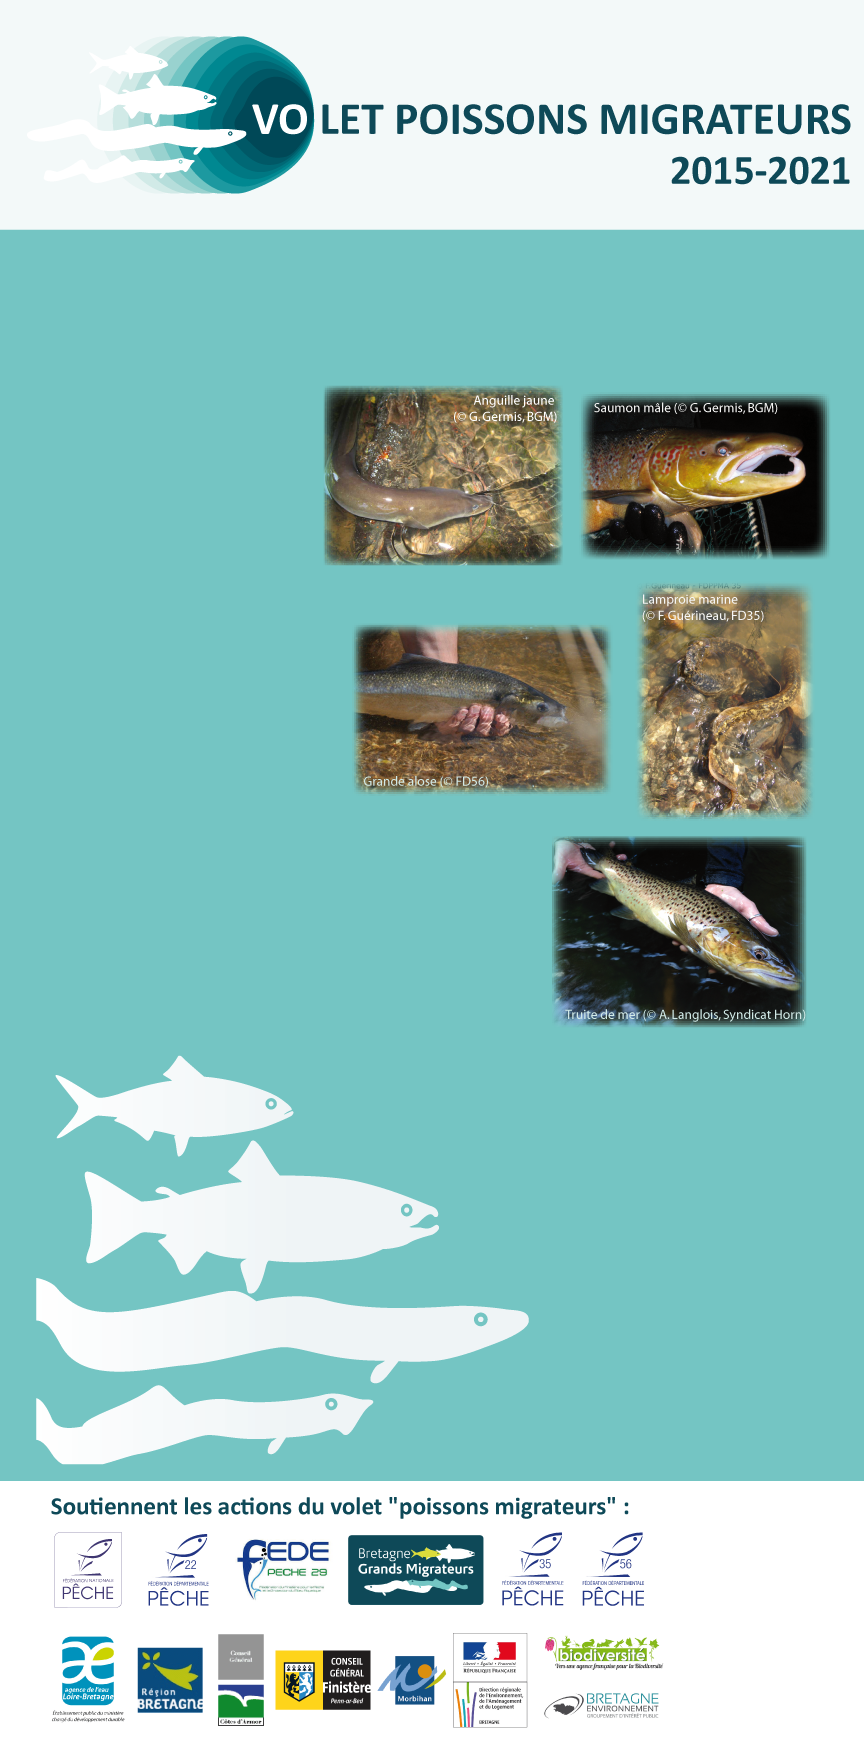
\includegraphics[%width=\paperwidth,
height=\paperheight,%
keepaspectratio]{/2023/frontpage.png}%
%\vfill
}}}%

\hfill%
\begin{minipage}{0.28\textwidth}

\par\sffamily\selectfont
\vspace{4cm}
\Large 
    {\titlefont Suivi scientifique des migrations de poissons 
    de la passe à bassins du barrage d'Arzal.
    Rapport 2023.}\\
\vspace{2cm}


\includegraphics[width=\textwidth]{/logo_EV} 
\end{minipage}
\vfill
\vspace{1.5cm}
\hfill%
\begin{minipage}{0.28\textwidth}
\textbf{
{\titlefont Date d'édition :\\}}
\qquad \color{orange_EV}
\Large
{\titlefont Mars 2024}
\vspace{2cm}

\end{minipage}

       
    
\hfill{ %
\begin{minipage}{0.28\textwidth}
\textbf{Réalisé avec le concours de} : \par
\vspace{1cm}
% le logo de l'agence doit au moins faire 25 mm de haut      
\centering{
\includegraphics[height=20mm]{/logo_agence.png}} 

\includegraphics[height=20mm]{/logo_region_bretagne.png}
\end{minipage}
}%  
\vfill
\hfill{ %
\begin{minipage}{0.3\textwidth}
\large
\color{bleu_EV}
\leftskip=1cm
Léa Patau\par
Cédric Briand\par   
Brice Sauvaget\par
Gérard Eriau\par
\vspace{1cm}
\end{minipage}
}% 
\endgroup
\end{titlepage}

%%%%%%%%%%%%%%%%%%%%%%%%%%%%%%%%%%%%%%%%%%%%%%%%%%%%%%%%%%%%%%%%%%%%%%%

\newpage
\newgeometry{right=1.5cm, left=1.2cm, top=0.2cm, bottom=2cm}
\thispagestyle{empty}
\pagecolor{bleu_EV}
\newgeometry{margin=0cm}
\begin{minipage}{\textwidth}
\vspace{30pt}
\hspace{30pt}

\includegraphics[width=6cm,keepaspectratio=true]{/logo_EV1}
\end{minipage}

%\vspace*{0cm}
\begin{minipage}{0.1\textwidth}
\phantom{This text will be invisible}
\end{minipage}
\begin{minipage}{0.8\textwidth}
\begin{center}
\noindent
{\color{turquoise_EV}\rule{\textwidth}{2.5pt}}\\
\vspace{8mm}
\color{white}
{ \titlefont \huge  \bfseries{Suivi scientifique des migrations de poissons 
    de la passe à bassins du barrage d'Arzal,\\
    }}
\bigskip
{\titlefont  \LARGE rapport 2023\par }
\vspace{4mm}\noindent
{\color{turquoise_EV}\rule{0.9\textwidth}{1.8pt}}\par
\vspace{5mm}
{\color{jaune_EV}{\titlefont \Large \itshape{Léa Patau, Brice Sauvaget,
      Gérard Eriau,
      Cédric Briand\par   }}}
\end{center}
\end{minipage}



\vspace{2cm}

\includegraphics[width=\paperwidth]{ala.png}

\vspace{2cm}
\begin{minipage}{0.8\textwidth}
\begin{center}
\hspace{3cm}{\color{white}{\huge \itshape{Janvier 2024}}}
\end{center}
\end{minipage}
\restoregeometry
\clearpage
\normalsize
\pagecolor{white}










  


\tableofcontents



%% Switch on the line numbers for the whole article at this place.
%\linenumbers


%% Main text is going here.

\bigskip



\section*{Introduction}
\label{Introduction}
L'estuaire de la Vilaine est limité à sa portion aval par le barrage d'Arzal,
construit par l'IAV en 1970, et qui bloque l'onde de marée à 10 km de
l'embouchure de l'estuaire.
L'estuaire en amont, jusqu'à la limite historique de l'estuaire tital (barrages de Malon et de la Potinais à 70-80 km en amont) 
a été transformé en rivière. Le plan d'eau ainsi créé a vu se développer de
nouveaux usages dont les principaux sont la navigation et
l'eau potable.
Le barrage d'Arzal joue un rôle majeur dans la protection contre les crues de l'aval du bassin versant, 
en empêchant les conjonctions de
forts débits amont et d'importantes surcotes de marées.
Ce barrage constitue ainsi une rupture nette entre des eaux saumâtres et douces. Il évacue le débit
de la Vilaine qui avec 12400 km$^2$ couvre le tiers de la surface la Bretagne.
Le barrage d'Arzal est un obstacle majeur à la circulation
des poissons migrateurs. Entre 1970 et 1995, année de la mise en service de dispositifs de franchissements,
leurs populations ont très fortement régressé sur le fleuve, voire même disparu.
Les passes à poissons du barrage d'Arzal, mises en service à l'automne 1995, 
font l'objet d'un suivi régulier. En 1996 et 1997, les migrations dans la passe à bassins 
ont été comptabilisées sur l'ensemble de l'année. Entre 1998 et 2012, seule la période favorable 
(généralement de mars à juin) fait l'objet d'un suivi. Depuis 2013, le suivi est à nouveau annuel. 


Ce rapport décrit le fonctionnement de la passe à fentes verticales du barrage
et de son système de vidéosurveillance associé. Il fait également la synthèse des passages de 
poissons migrateurs par la passe à bassins en 2023
\footnote{la migration sur les passes à anguilles est traitée dans un autre rapport :
\href{https://eptbvilaine56.sharepoint.com/:b:/g/extranet/ESZvGDLLuz9KiIVdrwVnVYoBQSDRPKLAm-CiNwjjwmFVjw?e=b6YyVl}{Gestion
de l'anguille sur le bassin versant de la Vilaine}.}.

   
    
\section{Matériel et méthodes}

\subsection{Site d'étude}
\subsubsection{Le barrage}

L’ouvrage, édifié entre 1965 et 1970, est constitué d’une partie centrale de 160 mètres comprenant 5 vannes 
et une écluse, et d’une digue en terre de 360 mètres (Photo
\ref{photo_barrage}).
Il bloque l’onde de marée à 12 kilomètres de l’embouchure et constitue une rupture nette entre le milieu estuarien 
et le plan d’eau douce artificiellement créé à l’amont. 
Le marnage à l’aval est de 7 mètres lors des grandes marées (Figure
\ref{photo_barrage}).

\begin{figure}[htpb]
\centering
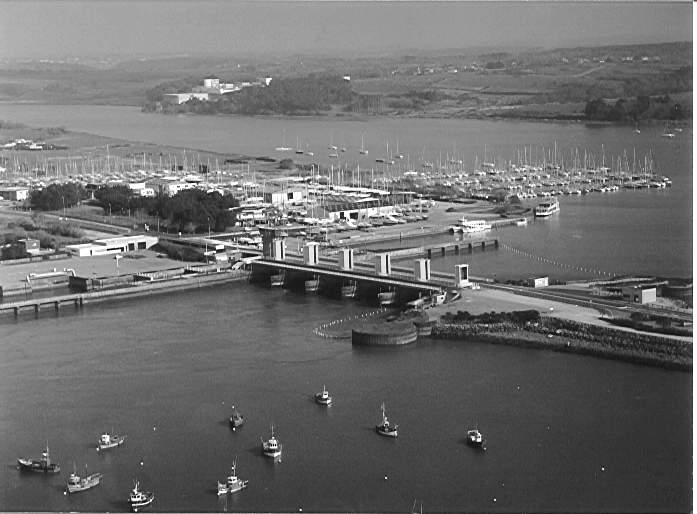
\includegraphics[width=0.45\textwidth]{barrage.png}
\caption{Photographie aérienne du barrage d'Arzal.
}
\label{photo_barrage}
\end{figure}


\subsubsection{La passe à bassins}

Deux passes ont été construites en 1995 sur le barrage. La première est un
dispositif spécifique pour les anguilles composé de rampes de reptation plongeant dans l'estuaire et
permettant aux anguillettes et aux civelles de grimper le long des rampes en
prenant appui sur des brosses, puis plus en amont d'un piège, un vivier de
stockage dans lequel les anguilles tombent après avoir franchi la rampe.
La deuxième est la passe à bassins successifs dont le suivi fait l'objet de ce
rapport.
Elle est composée de 9 bassins successifs reliés entre eux par des fentes
verticales \citep{larinier_passes_1999}.
Des chutes s’établissent entre les bassins et permettent de passer de la cote de l’estuaire à la cote du plan d’eau amont
(la passe constitue une sorte d’escalier hydraulique). Le poisson est attiré à
l’entrée de la passe par un courant d’eau douce. Il va remonter successivement
la chute aval et les différents bassins de la passe à poissons (2) pour se
retrouver à l’amont du barrage au niveau de la
chambre de visualisation (3) (Figure \ref{figure_passe_bassins}).

\begin{figure}[htpb]
\centering
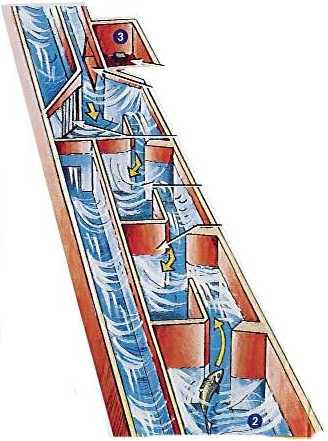
\includegraphics[width=0.35\textwidth]{passe_bassins.png}
\caption{Reconstitution pédagogique vue de dessus et en 3D de la passe à bassins du barrage d’Arzal.
}
\label{figure_passe_bassins}
\end{figure}

Les paramètres hydrauliques de la passe conditionnent le passage des espèces migratrices : le courant doit être suffisant
pour attirer le poisson vers l’entrée de la passe, mais pas trop puissant pour lui permettre de franchir les chutes
qui s’établissent entre chaque bassin. Ces paramètres doivent rester compris dans une gamme de valeurs permettant 
le franchissement des espèces que l’on désire faire passer. Ils dépendent étroitement du niveau d’eau amont et de
la hauteur de chute qui s’établit en entrée de passe. Or, le niveau aval, lié à
la marée, et le niveau amont lié à la gestion du plan d’eau par le barrage, sont très fluctuants. Une série de vannes gérées par un automate permet d’adapter en permanence 
le nombre de bassins (le nombre de marches d’escalier nécessaires pour franchir le dénivelé) et la hauteur de chute aval 
(la hauteur de la première marche). La mise au point de la passe a été réalisée en 1996 et a permis de caler les 
conditions de course, d’ouverture et de fermeture des différentes vannes en
fonction du niveau de la marée \citep{briand_suivi_1998}.
La passe à bassins est franchissable par plusieurs espèces marines, avec les grands migrateurs
(saumon, truite de mer, alose, lamproie, mulet, anguille jaune) et d’autres
espèces dont les passages sont anecdotiques (bar, flet), mais également par des espèces d’eau douce dévalant en estuaire par l’écluse 
ou par les vannes lors des épisodes de forts débits (silure, carpe, amour
blanc, sandre, gardon, ablette, brème ...). 
L'usage de bassins successifs séparés par des fentes verticales permet de
s’adapter aux grandes variations de niveaux amont et aval rencontrées en estuaire.


\subsection{Fonctionnement de la passe à bassins}
\subsubsection{Principe}
Le rôle du barrage d’Arzal est de limiter au maximum les entrées d’eau salée en Vilaine. La passe à bassins, 
située à l’interface de la mer et de l’eau douce, subit donc des contraintes liées aux marées.
Un automate informatique gère les vannes aval et amont de la passe à bassins en fonction des niveaux d’eau de la mer
et de la Vilaine. La passe fonctionne seulement quand le niveau de la mer est inférieur au niveau amont. 
La contrainte de sécurité de 30 cm sert à empêcher les intrusions d’eau salée dans le plan d’eau amont. 
La passe reste en fonctionnement à basse mer mais on considère qu’au-delà de 50 cm la chute à l’aval de la passe 
n’est plus franchissable. Lorsque le niveau dans le dernier bassin à l’aval de la passe (Niveau SAS) 
est situé 50 cm en dessus du niveau mer, la passe est considérée en dysfonctionnement hydraulique.
\subsubsection{Catégories d'état de la passe à bassins}
Les fonctionnements de la passe sont classifiés suivant les standards nationaux
établis par le SANDRE dans le
\href{http://www.sandre.eaufrance.fr/notice-doc/station-de-contrôle-des-migrations-de-poissons}{guide
des stations de contrôle des migrations} :
\begin{enumerate}
\item Fonctionnement normal.
\item Arrêt ponctuel lié au fonctionnement du dispositif : marée haute.
\item Arrêt technique : la passe est arrêtée mais compte tenu du niveau de la mer, elle pourrait être en fonctionnement. 
Les limitations de fonctionnement en période d’étiage sont inclues dans cette catégorie.
\item Dysfonctionnement hydraulique : à basse mer, la hauteur de chute à l’aval empêche la migration des poissons.
\item Inconnu : pas de données provenant de la base de données du barrage.
\end{enumerate}


%%%%%%%%%%%%%%%%%%%%%%%%%%%%%%%%%%%%%%%%
\begin{figure}[htpb]
\centering
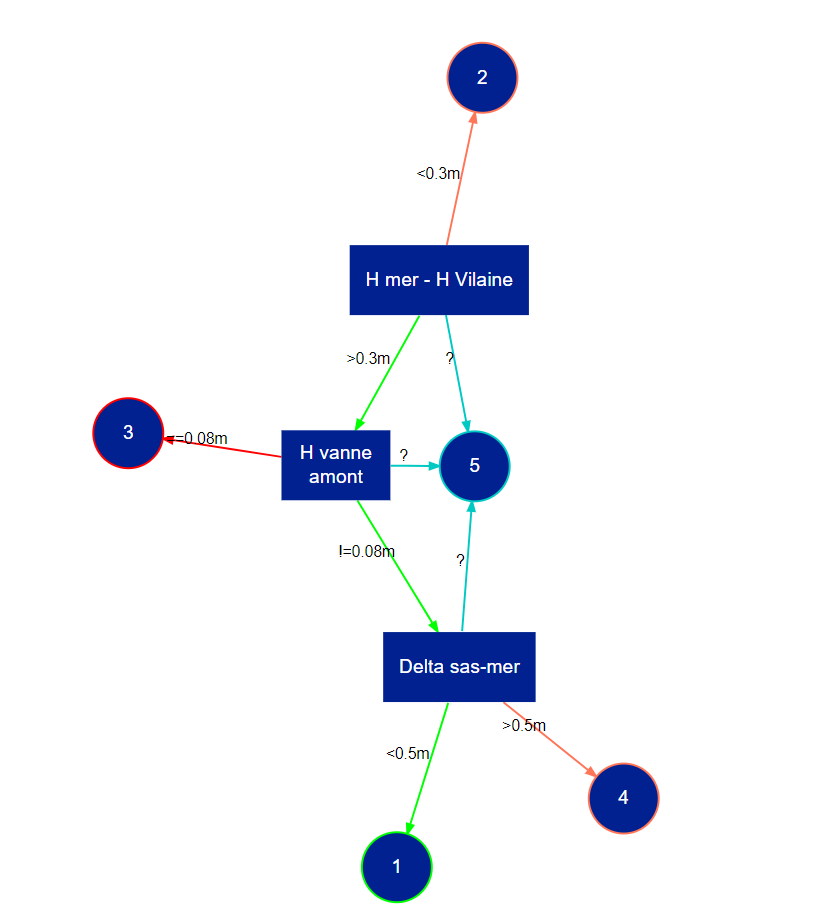
\includegraphics[width=0.5\textwidth]{schema_fonctionnement_EV.png}
\caption{Diagramme schématique de l'algorithme de calcul du fonctionnement de la
passe. Les valeurs sont en mètres. La passe fonctionne pour une différence de
niveaux entre la Vilaine et la mer supérieure à 0.3 m, elle est fermée quand le
codeur de la vanne amont est à la cote 0.08 m, elle est ouverte pour toutes les
autres valeurs.
Un dysfonctionnement hydraulique est noté pour des valeurs de chute aval
supérieures à 0.5 m (lors des basses mer). En cercles les types de
fonctionnement du dispositif, 1 = Fonctionnement normal, 2 = arrêt normal dû au fonctionnement du dispositif, ici marée haute, 3 =
arrêt pour maintenance, 4 = dysfonctionnement hydraulique, 5 pas de données. Le
graphique est créé à partir du package DiagrammeR
\citep{Iannone_diagrammer_2019}.}
\label{figure_schema_fonctionnement}
\end{figure}

En pratique, il est difficile de différentier un arrêt technique de la passe et
un arrêt à marée haute. Ainsi, les périodes d'arrêt technique de la passe sont
traduites en alternance de périodes d'arrêt technique, pendant lesquelles la
passe est fermée alors que le niveau de la mer permettrait son ouverture, et des
périodes d'arrêt normal liées au fonctionnement. Pour ces dernières en effet, en
fonctionnement normal la passe aurait été fermée car le niveau de la mer s'approche à moins de 30 cm du niveau de la Vilaine ce qui
aurait déclenché la fermeture de la vanne amont pour éviter les intrusions d'eau
salée (Figure \ref{detail_fonct_passe_2} en annexe).

En dehors des périodes d'arrêt et lorsque les coefficients de marée dépassent
70, la passe alterne entre des périodes où elle est fermée à marée haute, des
périodes de régulation à marée montante et descendante, et où le niveau de la
mer à basse mer descend en dessous de la cote de régulation de la vanne. La
chute aval augmente alors au delà du seuil de 50 cm auquel nous
considérons que la passe devient infranchissable (dysfonctionnement hydraulique) 
(Figure \ref{detail_fonct_passe_1} en annexe).


Lors des périodes d'étiages, deux moyens sont utilisés pour réduire le débit de
la passe. D'une part la fermeture du canal de débit d'appoint qui double
le débit dans le bassin aval de la passe, d'autre part l'arrêt de la passe
à basse mer car les migrations sont nulles lorsque la passe est en
dysfonctionnement hydraulique, et globalement les passages sont faibles
lors des marées descendantes et à basse mer. Malgré la baisse de débit, nous
considérons que la passe reste attractive car l'exutoire des tuyaux du siphon se situe près de l'entrée aval de la passe. 
De plus, il n'est pas nécessaire de maintenir un débit d'attrait important pour
que les poissons trouvent la source principale de l'eau douce s'écoulant dans l'estuaire dont la salinité
est proche de l'eau de mer en absence de débit.



\subsection{Système de suivi vidéo numérique}

Avant leur sortie à l'amont de la passe, les poissons sont dirigés par un
système de grille vers un couloir équipé de vitres. Un caisson de rétroéclairage
permet de filmer les poissons en ombres chinoises. Le système d'enregistrement
se compose d'une caméra, d'un ordinateur pour l'enregistrement (Figure
\ref{photo:suivi_numerique}). Le système de comptage est basé sur un enregistrement numérique des passages de poissons réalisé à l’aide des logiciels SYSIPAP (Système de Surveillance Informatisée 
des Passes à Poissons). Ce système fonctionne en deux phases :

\begin{itemize}
\item la première est une phase d'enregistrement sur le site de séquences vidéo
numérisées et compressées d’une taille d’environ 10 Mo (logiciel WSEQ32, vers. 6.2),
\item la deuxième est un dépouillement des enregistrements en temps différé
(WPOIS32, vers. 5.2).
\end{itemize}

\begin{figure}[htpb]
\centering
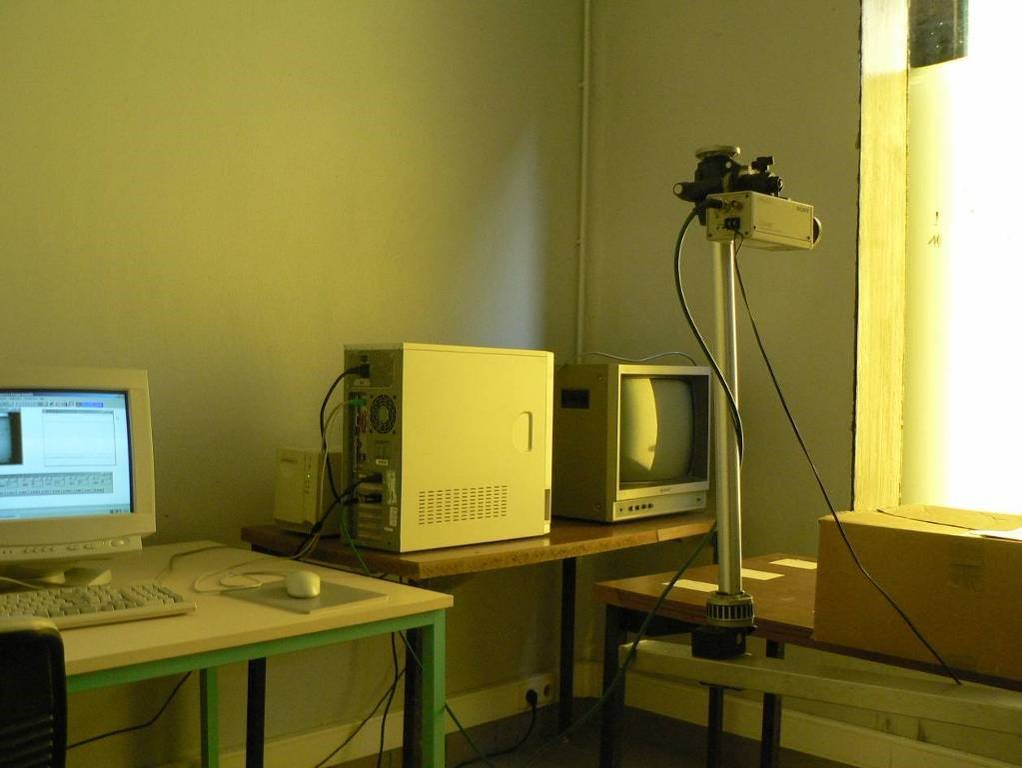
\includegraphics[width=0.45\textwidth]{suivi_numerique.jpg}
\caption{Système de suivi vidéo numérique.
}
\label{photo:suivi_numerique}
\end{figure}

\subsubsection{Enregistrement vidéo}
Le logiciel d'acquisition de séquences d'images WSEQ32 (Image
\ref{image:wseq32}) comprend les fonctionnalités suivantes :
\begin{itemize}
\item	déclenchement d'alarme basée sur la détection de variations d'intensité
lumineuse,
\item	déclenchement d'enregistrement comprimé sur le disque dur d'un PC.
\end{itemize}
Les paramètres ajustables sont :
\begin{enumerate}
\item	le cycle de mesure,
\item   la taille, la sensibilité et le mode actif/inactif des cellules
composant l'écran, 
\item	le seuil de déclenchement de l'alarme,
\item	la temporisation de l’alarme,
\item	le nombre d’images enregistrées précédant la condition de déclenchement.
\end{enumerate}

\begin{figure}[htpb]
\centering
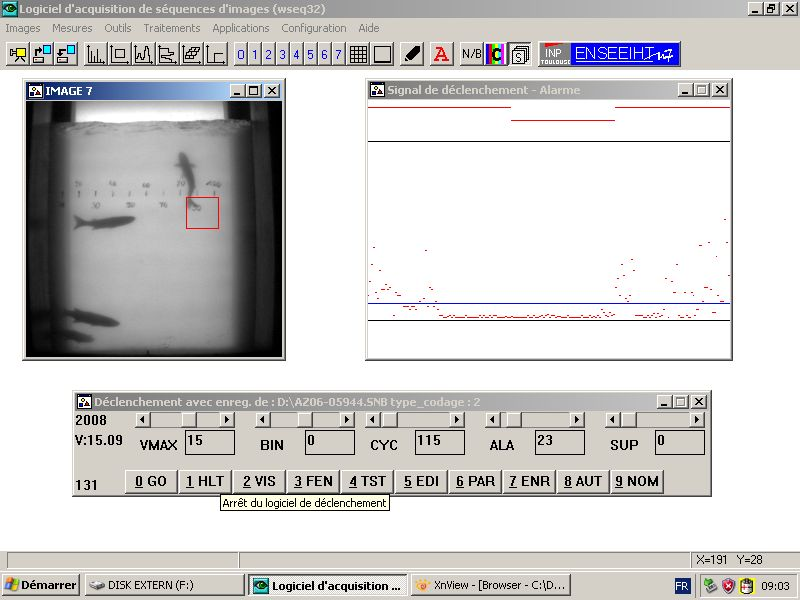
\includegraphics[width=0.45\textwidth]{wseq32.png}
\caption{Logiciel d’acquisition vidéo.
}
\label{image:wseq32}
\end{figure}

\subsubsection{Dépouillement vidéo}

Le logiciel de dépouillement WPOIS32 (Figure \ref{image:wpois32}) fonctionne sur Arzal de
manière manuelle, c'est-à-dire que la personne qui visionne les fichiers vidéo doit reconnaître
les différentes espèces et rentrer les effectifs correspondant à l’aide de l’interface "choix espèce".
Le résultat du dépouillement est un fichier texte comprenant la liste des événements enregistrés :
espèce, montée ou descente, numéro de l’image de sortie, date et heure, taille
en pixel et distance du poisson à la vitre.

\begin{figure}[htpb]
\centering
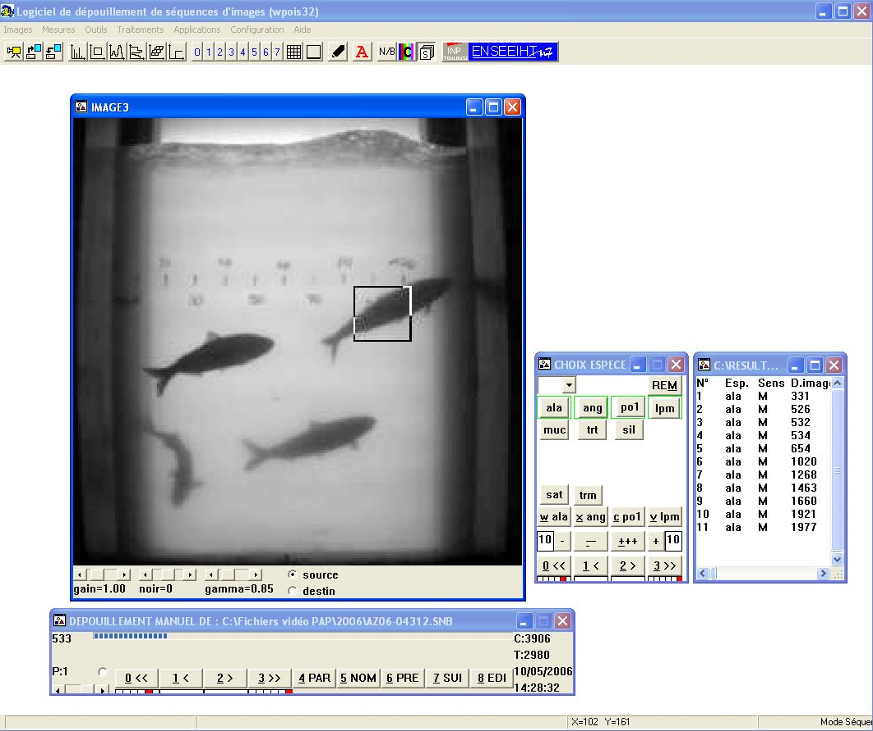
\includegraphics[width=0.45\textwidth]{wpois32.png}
\caption{Logiciel de dépouillement vidéo.
}
\label{image:wpois32}
\end{figure}

\subsubsection{Echappement au dispositif de franchissement}

Le barrage d’Arzal, par son faible dénivelé, reste franchissable par les volets,
par l’écluse, voire par les vannes wagons lorsque le dénivelé est faible. Mais
il ne l’est que dans certaines conditions et sur de courtes périodes.

La gestion du barrage, liée aux contraintes hydrauliques amont (débit à évacuer) et aval (marée), 
a une grande incidence sur la franchissabilité du barrage.
Le débit du fleuve peut être évacué par des vannes wagons ou
par des clapets flottants (volets) en surverse.
En règle générale, la plus grande part du débit est évacuée de jour, par l’intermédiaire des vannes. 
L’ouverture des volets la nuit permet de s’affranchir de la surveillance des vannes, 
les volets flottants empêchant mécaniquement la remontée de l’eau de mer dans le
plan d’eau amont. En période printanière quand les débits sont faibles et que
les volets fonctionnent, des bancs de mulets peuvent tenter de les franchir. Ce
franchissement peut concerner plusieurs milliers d'individus dans la demie heure
où les volets sont franchissables.

Entre 2013 et 2020 nous avons observé grâce à un sonar multifaisceaux (DIDSON)
des passages de lamproies marines sous les vannes lorsque les vitesses de courant ne sont pas élevées. Les effectifs recalculés peuvent être conséquents.
Lorsque la marée monte jusqu’au niveau des volets, il arrive un moment où ils sont franchissables par des espèces
ayant une bonne capacité de nage. Les chiffres donnés pour
l’évaluation des stocks de migrateurs doivent donc être considérés comme un minimum.

\section{Résultats}
\subsection{Fonctionnement de la passe à bassins}
\paragraph{Résumé du fonctionnement.}

Le fonctionnement de la passe en 2023 a été plutôt bon. 
La passe a été lancée le 1er février après une crue, puis arrêtée 
le 1er novembre avec la première crue automnale. La passe est en 
effet fermée en débit de crue pour empêcher la descente d'objets 
flottants et car la baisse de la ligne d'eau amont limite fortement les débits évacués.
La crue printanière du 9 mars au 2 avril a perturbé le fonctionnement 
de la passe mais sans entraîner d'arrêt. Il y a eu deux autres interruptions en cours de saison, 
du 16 au 18 août pour changer la sonde de niveau du SAS, et du 31 août au 5 septembre 
pour cause de submersion marine.

\begin{figure}[htpb]
\centering
\includegraphics[width=0.45\textwidth]{2023/fonctionnement_passe.png}
\caption{Fonctionnement de la passe en 2023, niveaux Vilaine, mer, sas
(dernier bassin en aval de la passe), et niveau de la vanne aval. Chaque point correspond aux niveaux
enregistrés lors d'une période de 10 minutes. Les données ont été corrigées des
valeurs abérrantes. Les données concernant le codeur du vérin de la vanne aval
sont manquantes en début de saison.}
\label{figure_fonctionnement_passe}
\end{figure}

\paragraph{Calculs du fonctionnement et des débits la passe à bassins.}
Les niveaux observés pour la ligne d'eau et les cotes de vannes de la passe
à bassins sont illustrés en Figure \ref{figure_fonctionnement_passe}. A
partir de ces niveaux, dont le détail est présenté en annexe (Figures
\ref{detail_fonct_passe_2} et \ref{detail_fonct_passe_1}), le fonctionnement
de la passe est calculé par période de 10 minutes (Figure \ref{report_df_annee}
en annexe).

En Figure \ref{report_df_fct_2003_2023}, l'analyse des durées mensuelles
cumulées de chaque type de fonctionnement permet de se donner une idée des
périodes auxquelles la passe a été arrêtée (en orange
\textcolor{orange_EV}{\rule[-0.2mm]{3mm}{2mm}}), mais également des périodes où elle a fonctionné de manière plus limitée, 
par exemple le passage en mode étiage de 2016 à 2019 se traduit par une  
augmentation de la durée des dysfonctionnements
(en orange \textcolor{orange_EV}{\rule[-0.2mm]{3mm}{2mm}}) ou par des arrêts
nocturnes (en jaune \textcolor{jaune_EV}{\rule[-0.2mm]{3mm}{2mm}}). Les mêmes
graphiques sont présentés pour la période 2003-2011 (Figure
\ref{report_df_2003_2023}) en mettant juste en avant les périodes où la passe est fonctionnelle
(en bleu \textcolor{bleu_EV}{\rule[-0.2mm]{3mm}{2mm}}) et les périodes où elle
ne l'est pas (en orange \textcolor{orange_EV}{\rule[-0.2mm]{3mm}{2mm}}).

Les débits de la passe calculés par l'automate du barrage 
(Figure \ref{debit_passe_mesure} en annexe) sont aussi recalculés en prenant en
compte des corrections de valeurs abérrantes et du coefficient de noyage de la vanne aval
(Figure \ref{debit_passe_calcul} en annexe, Figure \ref{debit_passe_comp}).

\begin{figure}[htpb]
\centering
\includegraphics[width=0.45\textwidth]{2023/debit_passe_comp.png}
\caption{Débits de la passe en 2023. Débits produits par l'automate du
barrage et recalculés en prenant compte du noyage de la chute à l'aval et des
valeurs abérrantes de niveaux.}
\label{debit_passe_comp}
\end{figure}

%
\begin{figure}[htpb]
\centering
\includegraphics[width=0.45\textwidth]{2023/report_df_fct_2003_2023.png}
\caption{Fonctionnement de la passe de 2003 à 2023, avec les détails par type
de fonctionnement.}
\label{report_df_fct_2003_2023}
\end{figure}%
%

%
\begin{figure}[htpb]
\centering
\includegraphics[width=0.45\textwidth]{2023/report_df_2003_2023.png}
\caption{Fonctionnement de la passe de 2003 à 2023.}
\label{report_df_2003_2023}
\end{figure}%
%

\paragraph{Fonctionnement du dispositif de comptage.}

Le dispositif de comptage a été mis en service le 6 février et arrêté le 3 novembre. 
Un long arrêt technique est intervenu du 31 août au 5 octobre à la suite 
d'une submersion marine qui a noyé le caisson lumineux et détruit les néons led.
Le délai pour se procurer les nouveaux néons a été très long.

\begin{figure}[htpb]
\centering
\includegraphics[width=0.45\textwidth]{2023/report_dc_2023.png} 
\caption{Bilan du fonctionnement du dispositif de comptage en 2023.}
\label{report_dc_2023}
\end{figure}

\begin{figure}[htpb]
\centering
\includegraphics[width=0.45\textwidth]{2023/report_dc_1998_2023.png} 
\caption{Bilan du fonctionnement du dispositif de comptage de 1998 à 2023.}
\label{report_dc_1998_2023}
\end{figure}
























%%%%%%%%%%%%%%%%%%%%%%%%%%%%%%%%%%%%%%%%%%%%%%%%%%%%%%%%%%%%%%%%%%%%%%%%%%%%%%%
\subsection{Conditions environnementales}

L'année 2023 a été marquée par des débits de crue en début et en
fin d'année et des débits globalement plus importants que les débits de
référence de la banque hydro (Figure \ref{fig_debit}).
\begin{figure}[htpb]
\centering
\includegraphics[width=0.45\textwidth]{2023/fig_debit.png} 
\caption{Débits de la Vilaine en 2023. En bleu les débits mesurés au Pont
de Cran, à l'aide d'une sonde à ultrasons, en orange les débits instantanés au
barrage d'Arzal (volets et vannes). Chaque point représente la valeur moyenne calculée toute les
dix minutes, noter l'absence de débit par les volets et les vannes en période
estivale. Les débits de référence mensuels moyens de la banque hydro au pont de
Cran sont donnés en marron.}
\label{fig_debit}
\end{figure}


\clearpage





\subsection{Mulet}
\makebox[-10pt]{ % decale vers le base par rapport 
  \begin{tikzpicture}[overlay]
  \node[inner sep=0pt] (muc) at (150pt,30pt)
      {
      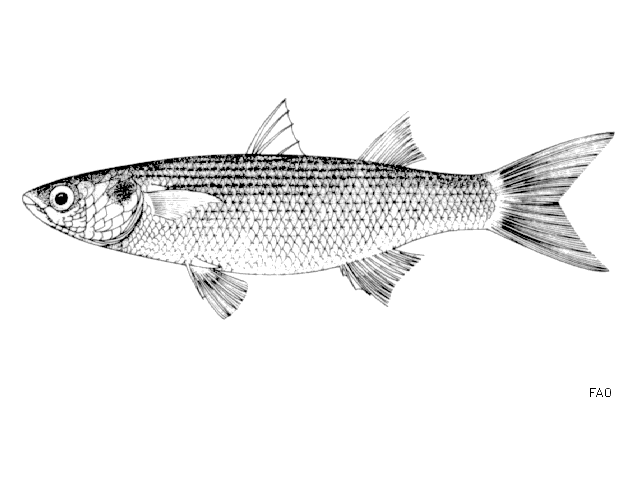
\includegraphics[width=.15\textwidth]{mulet.png}
      };
   \node[inner sep=0pt] (status) at (100pt,35pt)
      {
      
\includegraphics[width=0.5cm]{LC.jpg}
      };     
  \end{tikzpicture}
}
\fbox{\begin{minipage}[t]{0.48\textwidth}
\par\small
\titlefont\textcolor{bleu_EV}{
Le mulet porc \textit{Chelon ramada} est considéré en France comme
l’espèce de Mugilidés la plus ubiquiste tant en cours d’eau qu’en zône côtière
\citep{farrugio_biologie_1974,gautier_mulets_2005}. 
A partir du printemps, le mulet porc peut effectuer des migrations sur des longues distances 
entre les eaux marine et douce pour trouver des habitats favorables à sa
croissance. La reproduction a lieu fin
d'automne-début hiver, sur la zone littorale à proximité des estuaires. Il migre
donc à l'automne en avalaison sur les fleuves pour rejoindre le littoral.
Il fait l'objet d'une exploitation par la pêche professionnelle en Vilaine, 
et constitue après l'anguille la première espèce en effectif dans les comptages
aux passes à poissons du barrage d'Arzal.
En France les effectifs de mulet sont aujourd’hui en régression 
\citep{bartulovic_reproductive_2011}, l'espèce est néanmoins classée en
préoccupation mineure sur la liste rouge de l'IUCN.
Sur la Vilaine au barrage d’Arzal, parmi les mulets, seul \textit{Chelon
ramada} remonte l’estuaire pour migrer en eau douce \citep{briand_suivi_2018b}.
 En effet, le passage des poissons entre le milieu estuarien et le milieu de
 rivière provoque une variation brutale de salinité entre l'eau estuarienne et l'eau douce, 
 que seule \textit{Chelon ramada} pourrait supporter à l’aller et au retour de migration
 \citep{briand_suivi_2018b}.
 La présence de la seule espèce euryhaline et le confinement à la zone estuarienne 
 des autres espèces communes en Bretagne \textit{Chelon labrosus} et \textit{Chelon aurata}
 est cependant à confirmer \citep{gautier_mulets_2005,trancart_analyse_2011}.}
 \end{minipage}}
\smallskip



Compte tenu des effectifs très importants de mulets franchissant le barrage
d'Arzal chaque année, les comptages n'ont pas été effectués sur l'ensemble de la
période de suivi historique de la passe. Ils ont été effectués en 1996 et
1997, en 2013, 2005 et de 2013 à 2023. Lors des pics de migration, le comptage
des mulets est effectué par lots de 10 individus en cas de forts passages, et la taille des poissons est analysée
sur des échantillons hebdomadaires.
La structure en
taille des mulets présente à la fois des variations saisonnières et
interannuelles (Figure \ref{figure_taille_mulets}). Les mulets les plus grands
se présentent en tout début de saison, puis la taille des mulets diminue pour
atteindre son minimum lors de l'été \citep{lemonnier_dynamique_2019}.
Cette année comme en 2019 les mulets de petite taille, qui constituent une
majeure partie des effectifs, ne sont pas présents, sans que le fonctionnement
de la passe puisse expliquer cette absence.

\begin{figure}[htpb]
\centering
\includegraphics[width=0.45\textwidth]{2023/graphe_taille_mulets.pdf} 
\caption{Tendance saisonnière d'évolution des
tailles de mulets depuis 2013. A. Graphiques de densités (distributions) des
tailles par mois, en jaune mois estivaux, en violet mois printaniers, en rose
automne. B. Graphique en violon et box-plot des tailles annuelles. C. Modèle gam
ajusté sur les valeurs de taille (au centre modèle et intervalle de confiance
 à 95 \%) les points correspondent à prédiction + résidus.}
\label{figure_taille_mulets}
\end{figure}



\begin{figure}[htpb]
\centering
\includegraphics[width=0.45\textwidth]{2023/bilan_annuel_mup2} 
\caption{Bilan annuel des migrations de mulets au barrage d'Arzal, pour
l’année complète et pour la période de montaison jusqu’au 31 août.}
\label{bilan_annuel_mup}
\end{figure}

Les effectifs de mulets de 2023
(N=102972) 
sont faibles comparés à ceux de la période 2014-2023 avec des variations entre
des effectifs de 200~000 à 600~000 mulets.
Les variations des effectifs de petits mulets sont en 
grande partie liée à l'abondance des mulets de classe de taille de 200 à 300 mm
\citep{lemonnier_dynamique_2019} (Tableau \ref{table_bilanannuel_mulets_0108}, Figure
\ref{bilan_annuel_mup}).

A partir de septembre, on note une augmentation des effectifs de mulets dans la
passe (Figure \ref{rmi_journalier_mup}) et les bancs de mulets commencent à
descendre la Vilaine pour retourner en mer participer à leur reproduction
annuelle. Les mulets peuvent alors faire des remontées dans la passe et la
structure en taille des mulets réaugmente en général en fin de saison. Les
raisons de la remontée à l'automne des mulets dans la passe ne sont pas connues,
mais le passage brutal de l'eau douce à l'eau salée en estuaire nécessite
probablement un temps d'adaptation pour effectuer la régulation osmotique.
Ainsi, les chiffres de migration totale représentent probablement un biais dans
l'interprétation de la taille de la population de mulets en Vilaine et un calcul
du nombre de mulets migrant jusqu'au mois de septembre (exclu) est donné au
Tableau \ref{table_bilanannuel_mulets_0108}.


%\input{vvv[["MUP"]][["path"]]} % table_bilanannuel_mulets
\input{C:/workspace/passe_bassins/table/2023/5_2183_IND_1996to20230108.tex} % table_bilanannuel_mulets

La migration des mulets
est essentiellement diurne et matinale (Figure \ref{horaires_mulet}) et elle
dépend également du niveau mer avec une grande part des passages pour des niveaux mer
>0m (Figure \ref{horaires_maree_mulet}).

\begin{figure}[htpb]
\centering
\includegraphics[width=0.45\textwidth]{2023/horaires_mulet} 
\caption{Horaires de migration des mulets en 2023.}
\label{horaires_mulet}
\end{figure}

% latex table generated in R 4.1.2 by xtable 1.8-4 package
% Fri Mar 11 14:20:24 2022
\begin{table}[htbp]
\centering
\begin{tabular}{lrrrr}
  \hline
Mois & Min* & Moyenne* & Max* & N (2021) \\ 
  \hline
févr. & 25 484 & 25 484 & 25 484 & 25 484 \\ 
  mars & 280 & 37 212 & 128 414 & 41 777 \\ 
  avr. & 162 & 55 020 & 105 678 & 88 634 \\ 
  mai & 29 738 & 73 504 & 150 324 & 45 600 \\ 
  juin & 12 783 & 59 646 & 211 779 & 13 370 \\ 
  juil. & 2 685 & 35 711 & 114 971 & 2 822 \\ 
  août & 6 164 & 19 203 & 41 156 & 6 164 \\ 
  sept. & 11 661 & 30 737 & 53 780 & 21 694 \\ 
  oct. & 402 & 40 732 & 114 637 & 10 689 \\ 
  nov. & -2 096 & 11 567 & 65 619 & 950 \\ 
  déc. & 5 & 5 & 5 & 5 \\ 
   \hline
\end{tabular}
\caption{Migrations mensuelles des mulets dans la passe à bassins du barrage d'Arzal, $N$ nombre, * correspondent à
				la période 1996-2021. min* minimum mensuel, max* maximum mensuel, moyenne* moyenne des effectifs mensuels.} 
\label{table_lpm_mois}
\end{table}


\begin{figure}[htpb]
\centering
\includegraphics[width=0.45\textwidth]{2023/bmm_horaires_maree} 
\caption{Passage des mulets par pas de temps de 10 minutes en fonction de
l'heure et du niveau mer en
2023.}
\label{horaires_maree_mulet}
\end{figure}


\clearpage
\onecolumn

\begin{landscape}
\begin{figure}[htpb]
\centering
\includegraphics[width=0.9\linewidth,keepaspectratio]{2023/rmi_journalier_mup.png} 
\caption{Bilan annuel des migrations de mulets \textit{Chelon ramada} au barrage
d'Arzal.}
\label{rmi_journalier_mup}
\end{figure}
\end{landscape}




















\clearpage
\twocolumn
\subsection{Lamproie marine}
%\vspace{5pt} % utiliser innertopmargin
\makebox[-10pt]{
  \begin{tikzpicture}[overlay]
  \node[inner sep=0pt] (lpm) at (150pt,30pt)
      {
      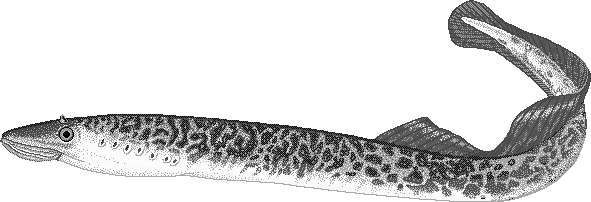
\includegraphics[width=.12\textwidth]{lpm.png}
      };
  \node[inner sep=0pt] (status) at (100pt,28pt)
      {
      
\includegraphics[width=0.5cm]{EN.jpg}
      };        
  \end{tikzpicture}
}
\fbox{
\begin{minipage}[t]{0.48\textwidth}
\par\small
\titlefont\textcolor{bleu_EV}{
Les lamproies \textit{Petromyzon marinus} sont des vertébrés primitifs de
la classe des Agnathes (sans mâchoire, avec une bouche circulaire), 
et ne sont donc pas à proprement parler des poissons. La lamproie marine est une espèce amphihaline. 
Elle ne se reproduit qu'une seule fois en eau douce en mai-juin, avec un homing
\footnote{\textcolor{bleu_EVf}{retour à la rivière de naissance}} faible.
Les larves ammocètes vivent enfouies dans les sédiments et les litières pendant 5 à 7 ans.
Après métamorphose, les lamproies dévalent en mer où elles vivent 1 à 2 ans en tant que parasite externe
sur des poissons ou des mammifères.
Au niveau national, la tendance des abondances est à la baisse, surtout sur les
sites qui étaient les plus fréquentés (Gironde, Loire), alors qu'en Bretagne, la chute est moins marquée. 
La contribution de la Vilaine à l'échelle de la France, très faible aux débuts des années 2000, 
est aujourd'hui non négligeable. Sur la Vilaine, les migrations de 2016 à 2019 
ont été très mauvaises, mais les saisons 2020 et 2023 marque un retour à la
normale.
L'espèce est classée en danger en France sur la liste rouge UICN.}
\end{minipage}}
\smallskip



Les migrations de lamproies marine sur la Vilaine qui étaient en fort déclin
après 2015 ont réaugmenté à un niveau proche du niveau historique
(N=\textcolor{orange_EV}{\num{3111}}) en 2020.
Cette année, les effectifs ont été de nouveau relativement faibles avec 
\textcolor{orange_EV}{\num{1150}} lamproies marines (Figure \ref{barplot_report_annual_lpm}, Tableau \ref{table_bilanannuel_lpm}) ce qui place l'année au \textcolor{orange_EV}{\num{14}} ème rang sur les
\textcolor{orange_EV}{\num{28}} années de suivi à Arzal.
Les raisons des variations d'effectif restent mal comprises.


		
\begin{figure}[htpb]
\centering
\includegraphics[width=0.45\textwidth]{2023/barplot_report_annual_lpm.png} 
\caption{Histogramme des effectifs annuels de lamproies marines comptabilisés
au barrage d'Arzal.}
\label{barplot_report_annual_lpm}
\end{figure}


La comparaison des tendances mensuelles avec les migrations
interannuelles montre qu'elles sont inférieures à la moyenne observée sur la
période 1996-2022 (Figure \ref{barchart_bmi_lpm}, Tableau
\ref{table_lpm_mois}).

\begin{figure}[htpb]
\centering
\includegraphics[width=0.45\textwidth]{2023/barchart_bmi_lpm.png} 
\caption{Comparaison de la migration de lamproies marines de 2023 avec la
série interannuelle de données 1996-2022.}
\label{barchart_bmi_lpm}
\end{figure}



% latex table generated in R 4.1.2 by xtable 1.8-4 package
% Mon Mar 07 15:07:02 2022
\begin{table}[htbp]
\centering
\begin{tabular}{lrrrr}
  \hline
Mois & Min* & Moyenne* & Max* & N (2021) \\ 
  \hline
  févr. & 1 & 2 & 2 & 1 \\ 
  mars & 1 & 66 & 220 & 220 \\ 
  avr. & 4 & 616 & 2 317 & 556 \\ 
  mai & 9 & 941 & 3 080 & 748 \\ 
  juin & 1 & 87 & 281 & 17 \\ 
   \hline
\end{tabular}
\caption{Migrations mensuelles des lamproies marines dans la passe à bassins du barrage d'Arzal, $N$ nombre, * correspondent à
				la période 1996-2021. min* minimum mensuel, max* maximum mensuel, moyenne* moyenne des effectifs mensuels.} 
\label{table_lpm_mois}
\end{table}
 % table bilan annuel lamproies
\input{C:/workspace/passe_bassins/table/2023/5_2014_11_1996to2023.tex} % table bilan lamproies pour l'année


La migration des lamproies marines intervient entre mars et juin (Figure
\ref{rmi_density_lpm}). En 2023, la migration s'est faite essentiellement
de mars à mai. Les premières migrations sont plus précoces que ce que l'on pensait,
et le suivi était souvent lancé trop tardivement avant 2021 
(1ère quinzaine de mars entre 2010 et 2020) pour voir les premiers individus
(Figures \ref{barchart_bmi_lpm}, \ref{plot_seasonal_lpm}).
Ces résultats sont en accord avec l'examen des tendances de migration des
lamproies marines en France par \citet{legrandContrastingTrendsSpecies2020} qui
montre globalement une arrivée plus précoce dans les 30 dernières années. 
Les dates de première arrivée (correspondant à l'arrivée de 5 \% des
effectifs annuels), arrivée médiane (quand 50 \% des lamproies ont migré) et
arrivées tardives (95 \%) ne varient pas de manière indépendante pour la
lamproie. 

\begin{figure}[htpb]
\centering
\includegraphics[width=0.45\textwidth]{2023/rmi_density_lpm.png} 
\caption{Saisonnalité de la migration des lamproies marines, les pourcentages
par quinzaine sont cumulés.}
\label{rmi_density_lpm}
\end{figure}


\begin{figure}[htpb]
\centering
\includegraphics[width=0.49\textwidth]{2023/plot_seasonal_lpm.png} 
\caption{Saisonnalité de la migration des lamproies marines, effectifs
hebdomadaires. Les
barres représentent le 5 ème et le 95 ème percentile de la migration. Le
point la médiane. L'importance des effectifs est représentée par la couleur.}
\label{plot_seasonal_lpm}
\end{figure}

La comparaison des structures en taille vidéo laisse
paraître un accroissement depuis 2015. C’est à partir de 2019 qu’une nouvelle méthode de
mesure a été appliquée : la taille a été mesurée relativement à 9 sections de la vitre de comptage pour
prendre en compte les déformations de la lentille
de la caméra. Or l’aumentation est observée depuis
2015, elle ne peut donc pas être attribuée au changement de méthode de mesure. L’augmentation de la
taille des lamproies est donc un phénomène notable,
comme pour les variations d’effectifs, les raisons de
cette augmentation de taille ne sont pas connues, et un phénomène exactement
similaire avait été rapportée sur la Loire (Marion Legrand, comm. pers.).
Cependant, pour l'année 2023, comme pour l'année précédente, les tailles des
lamproies sont en baisse par rapport aux années 2019, 2020 et 2021 (Figure \ref{size_lpm}).

\begin{figure}[htpb]
\centering
\includegraphics[width=0.45\textwidth]{2023/size_lpm.png} 
\caption{Comparaison des structure en taille des lamproies marines. Les tailles
de 2019 et 2023 ont été calculées en prenant en compte la déformation des distances dans les
différentes zones de la vitre.}
\label{size_lpm}
\end{figure}


%%%%%%%%%%%%%%%%%%%%%%%%%%%%%%%%%%%%%%%%%%%%%%%%%%%%%%%%%%%%%%%%%%%%%










\clearpage
\subsection{Aloses}

%\vspace{5pt} % utiliser innertopmargin
\makebox[-2.5pt]{
  \begin{tikzpicture}[overlay]
  \node[inner sep=0pt] (alose) at (150pt,30pt)
      {
      \begin{turn}{0}
      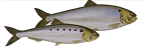
\includegraphics[width=.12\textwidth]{aloses.png}
      \end{turn}
      };
  \node[inner sep=0pt] (status) at (100pt,28pt)
      {
      
\includegraphics[width=0.5cm]{CR.jpg}
      };    
  \end{tikzpicture}
}
\fbox{\begin{minipage}[t]{0.48\textwidth}
\par\small
\titlefont\textcolor{bleu_EV}{Poisson migrateur amphihalin de la famille des
Clupéidés (sardine …).
La grande alose \textit{Alosa alosa} ne se reproduit généralement qu'une seule
fois, en eau douce en mai-juin, souvent sur sa rivière d'origine ou dans un cours d'eau 
proche géographiquement. Les alosons restent à proximité des frayères quelques mois 
avant de dévaler en automne vers l'estuaire, puis rapidement en mer pour une phase 
de croissance d'environ 5 ans. Les femelles sont plus massives que les mâles et restent 
généralement une année de plus en mer.
Au niveau national, la tendance est à une chute très marquée, 
surtout sur les sites qui étaient les plus fréquentés (Gironde, Loire).
En Bretagne, la situation est plutôt à l'amélioration, et la Vilaine fait partie
des principaux sites avec le Blavet et l'Aulne. Après la période 2012-2016 où 
la pêche professionnelle estuarienne a fortement impacté la migration, on a
constaté un renforcement des effectifs sans toutefois jamais atteindre les
valeurs historiques des années 2000. Les effectifs sont de nouveau en baisse sur
la Vilaine. L'espèce est classée en danger critique d’extinction en France sur
la liste rouge UICN.
}
\end{minipage}}
\smallskip

538 aloses ont été comptées en
2023 (Figure
\ref{rmi_journalier_ala} et \ref{tx_exploit}  et Tableau
\ref{table_bilanannuel_ala}).
Cette migration place l'année 2023 au rang 18
par rapport à l'ensemble des années de migration. En
vidéo comptage, il n'est pas possible de distinguer les deux espèces, grande
alose \textit{Alosa alosa} et alose feinte \textit{Alosa fallax}.


%\begin{figure}[htpb]
%\centering
%\includegraphics[width=0.45\textwidth]{2023/bilan_annuel_ala.png} 
%\caption{Histogramme des effectifs annuels d'aloses comptabilisés
%au barrage d'Arzal.}
%\label{bilan_annuel_ala}
%\end{figure}

\input{C:/workspace/passe_bassins/table/2023/5_2055_11_1996to2023.tex} 


\begin{figure}[htpb]
\centering
\includegraphics[width=0.45\textwidth]{2023/rmi_journalier_ala.png} 
\caption{Comparaison de la migration d'aloses de 2023 avec la série
interannuelle de données 1996-2022.}
\label{rmi_journalier_ala}
\end{figure}


Globalement, les migrations sont inférieures à la
moyenne interannuelle (Figures
\ref{rmi_journalier_ala} et \ref{barchart_bmi_ala}, Tableau \ref{table_ala_mois}).

\begin{figure}[htpb]
\centering
\includegraphics[width=0.45\textwidth]{2023/barchart_bmi_ala.png} 
\caption{Comparaison de la migration d'aloses de 2023 avec la série
interannuelle de données 1996-2022.}
\label{barchart_bmi_ala}
\end{figure}

La comparaison des structures en taille vidéo de cette année laisse apparaître
une forte diminution de la taille moyenne après une tendance sur plusieurs
années à l'augmentation.
A compter de 2019, la taille a été mesurée relativement à 9 zones de la vitre de
comptage pour prendre en compte les déformations de la lentille de la caméra. Ainsi les tailles avant 2019 et 2023
sont peut être légèrement plus petites (Figure \ref{size_alose}).
La diminution de la taille moyenne en 2020 semblait cohérente avec un retour des
premières aloses ayant fait l'objet de mesures de protection 5 ans auparavant en
2015, et la relative rareté des grandes aloses correspondant à la période de
surexploitation en 2012-2014. En 2021, les tailles avaient ré-augmenté,
puis elles diminuent depuis 2022. Ces variations de tailles moyennes
pourraient s'expliquer par des années pour lesquelles le succès reproducteur
serait plus faible, ou par la contribution plus ou moins importante d'aloses
provenant d'autres bassins.



\begin{figure}[htpb]
\centering
\includegraphics[width=0.45\textwidth]{2023/size_alose.png}
\caption{Taille des aloses mesurées à Arzal. Densité (graphique en violon),
moyenne et +- 2 fois l'écart type (en bleu foncé). La couleur des points dépend
du mois de passage.}
\label{size_alose}
\end{figure}


Contrairement à l'année 2019, le début de la migration n'est pas
particulièrement précoce (Figure \ref{plot_seasonal_ala}).




\begin{figure}[htpb]
\centering
\includegraphics[width=0.49\textwidth]{2023/plot_seasonal_ala.png} 
\caption{Saisonnalité de la migration des aloses, effectifs hebdomadaires. Les
barres représentent le 5 ème et le 95 ème percentile de la migration, le point
la médiane. L'importance des effectifs est représentée par la couleur.}
\label{plot_seasonal_ala}
\end{figure}

Depuis 2018, on considère qu'il n'y a pas eu d'exploitation
estuarienne de l'alose (Figure \ref{tx_exploit}). La gestion de la population d'aloses
de Vilaine a fait l'objet d'un
débat technique dans le cadre du Comité de gestion des poissons migrateurs de
Bretagne.
A partir des éléments collectés sur le bassin, et des données obtenues sur les
bassins voisins, un objectif de gestion en biomasse a été défini. Le
stock potentiel sur la Vilaine est estimé entre 50~000 aloses, pour
le niveau actuel d'aménagement du bassin - c'est à dire un fort étagement
par le barrage d'Arzal puis par les ouvrages de l'Oust et de la Vilaine- , et
100~000 aloses pour une rivière en conditions pristine, c'est à dire une
rivière pour laquelle l'accès aux zones de frayères serait restauré. Une limite
en biomasse, celle en-dessous de laquelle on estime qu'il pourrait y avoir un
risque accru de diminution du stock, est proposée à 15~000 aloses. En dessous de
cette limite, la mortalité devrait être réduite pour remonter le stock à son
niveau optimal. Une règle de gestion a été proposée pour la gestion des
pêcheries. L'importance de l'aménagement des axes fluviaux pour l'accès aux
zones de reproduction a également été mise en avant (Figure \ref{tx_exploit}).

La question de la prédation du silure, dont les effectifs
sont en claire augmentation avec des tailles allant en s'accroissant, devra se poser l'année
prochaine si les effectifs n'augmentent pas.


\vfill
\begin{figure}[pbt]
\centering
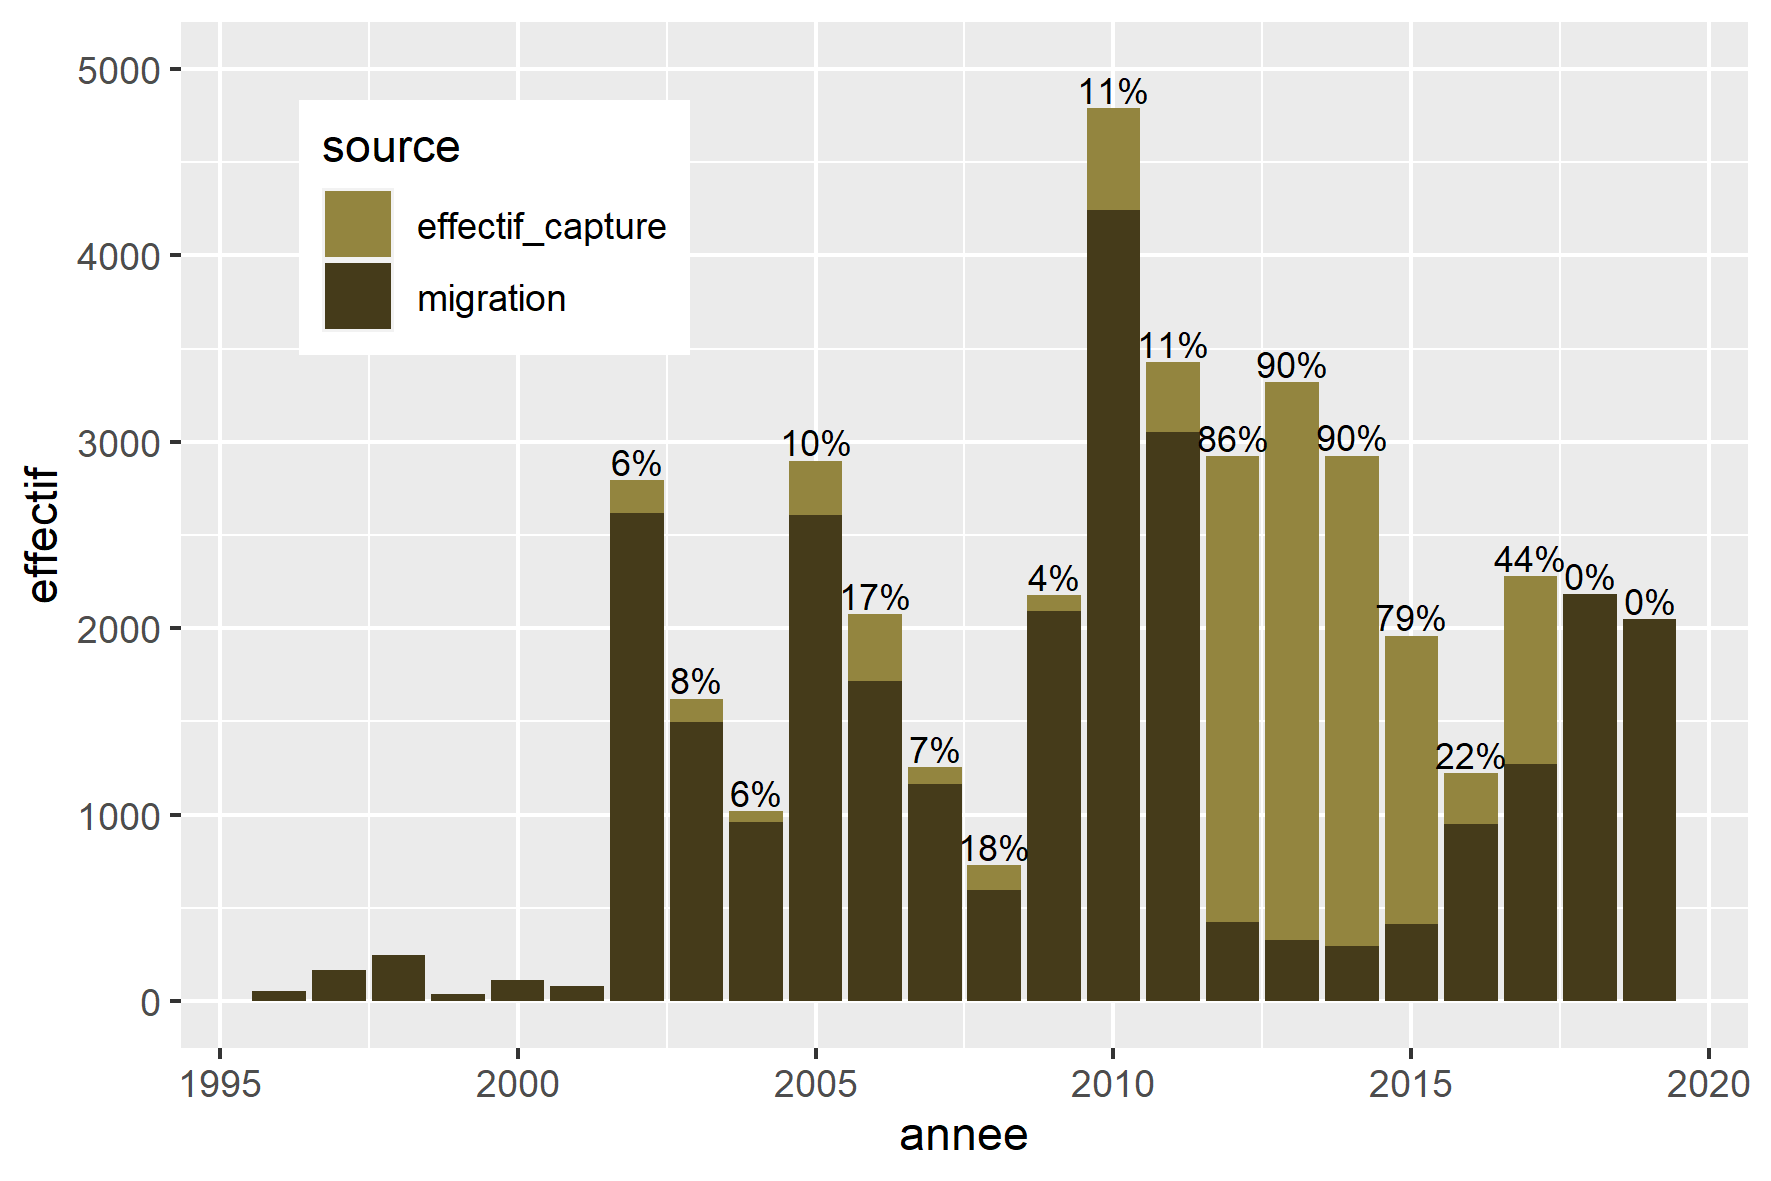
\includegraphics[width=0.5\textwidth]{2023/tx_exploit.png} 
\caption{Migration et taux d'exploitation des aloses en estuaire de Vilaine,
illustration de l'effet des mesures prises à partir de 2015 pour limiter
l'exploitation de l'espèce en estuaire. Interdictions par zones et saisonnières
de 2015 à 2017, puis interdiction totale saisonnière de pêche à partir de 2018.}
\label{tx_exploit}
\end{figure}
\newpage % column break

\input{C:/workspace/passe_bassins/table/2023//2055_IND_11_2016_2023.tex} % tableau avec effectifs mensuels 

\clearpage %
\begin{landscape}
\begin{figure}[htpb]
\centering
\includegraphics[width=0.9\linewidth]{2023/preco_diagram.png} 
\caption{Diagramme de précaution pour la gestion des aloses en Vilaine, 
les données indiquent la position du stock par rapport à la règle de gestion proposée 
par le groupe de travail du cogepomi sur les aloses. 
En abscisse, nombre de géniteurs par rapport à la cible de gestion, 
en ordonnée, mortalité cumulée (taux instantané) de la pêcherie estuarienne. 
Les données de la pêcherie fluviale, indisponibles, ne sont pas intégrées au
calcul.}
\label{preco_diagram}
\end{figure}
\end{landscape}



















\clearpage
\twocolumn
\subsection{Saumon atlantique}
%\vspace{5pt} % utiliser innertopmargin
\makebox[-2.5pt]{
  \begin{tikzpicture}[overlay]
  \node[inner sep=0pt] (alose) at (150pt,30pt)
      {
      \begin{turn}{0}
      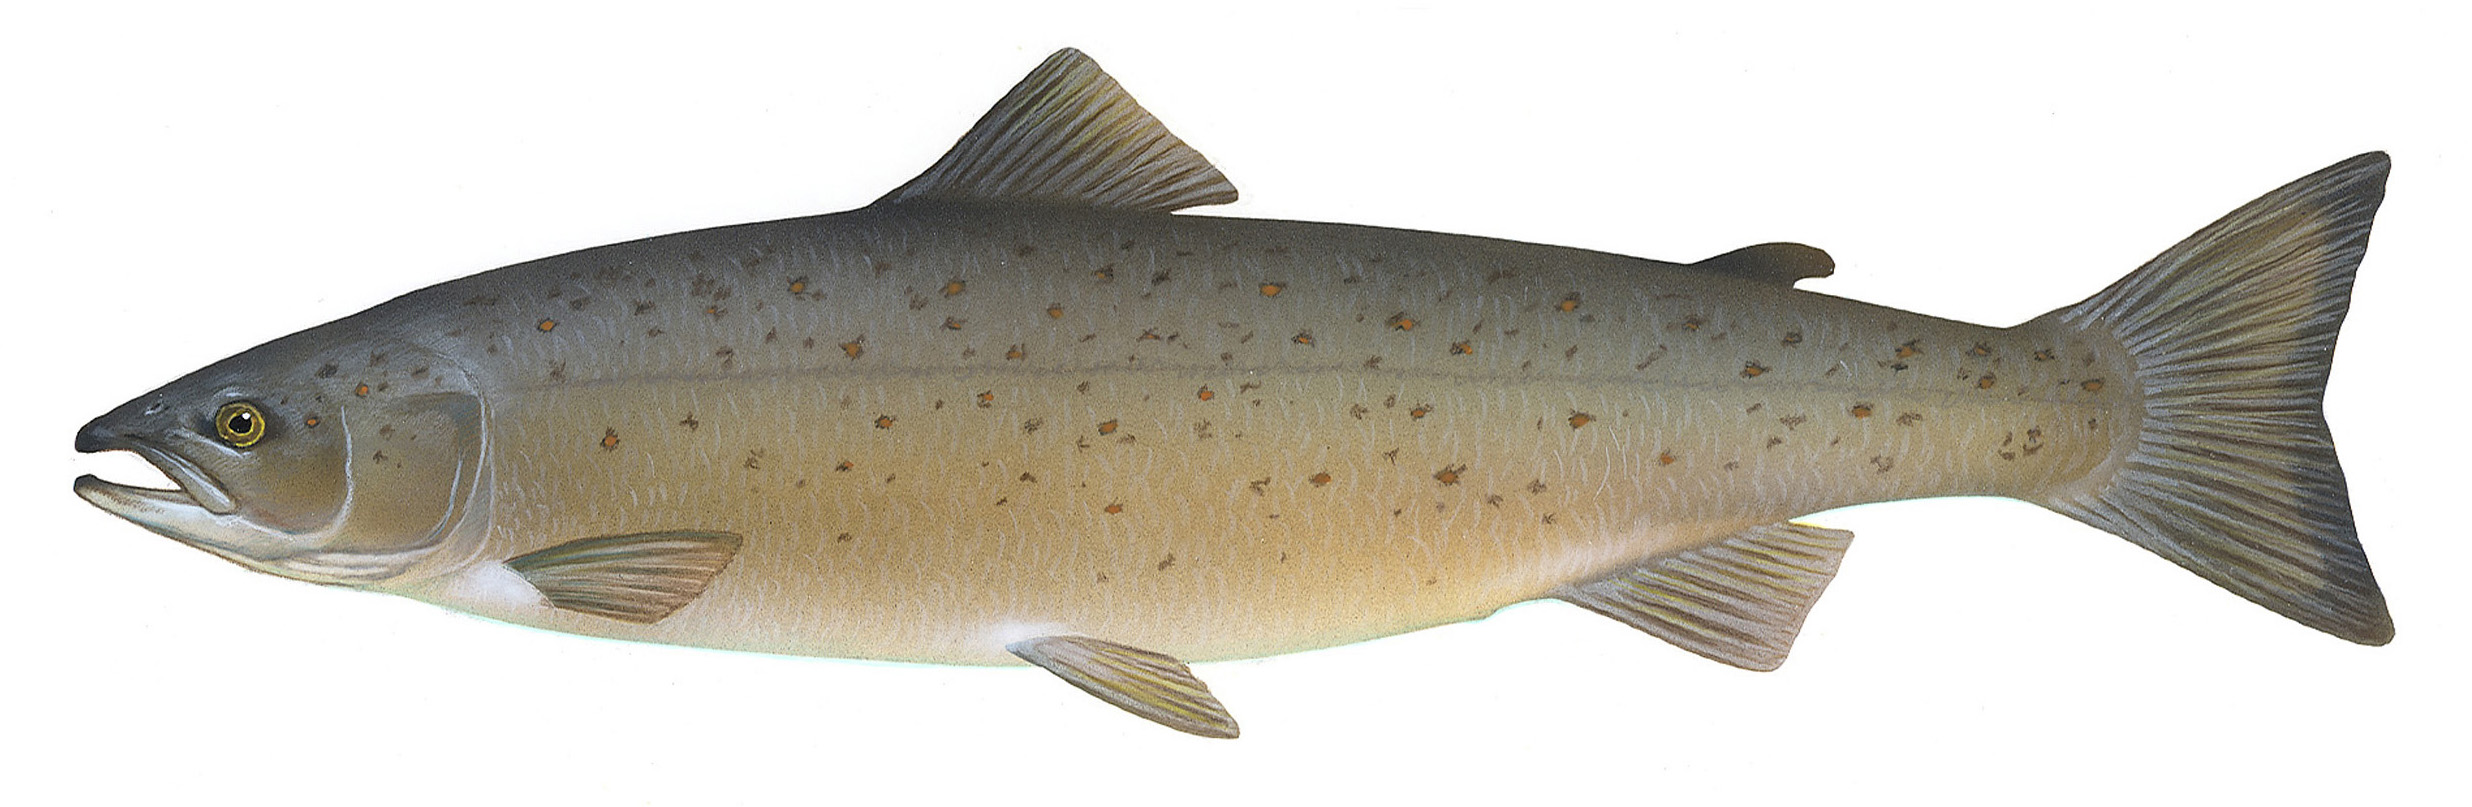
\includegraphics[width=.12\textwidth]{Salmo_salar.jpg}
      \end{turn}
      };
  \node[inner sep=0pt] (status) at (100pt,28pt)
      {
      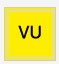
\includegraphics[width=0.5cm]{VU.jpg}
      };    
  \end{tikzpicture}
}
\fbox{\begin{minipage}[t]{0.45\textwidth}
\par\small
\titlefont\textcolor{bleu_EV}{
Le saumon atlantique \textit{Salmo salar} est un poisson migrateur amphihalin,
qui ne se reproduit généralement qu'une seule fois.
La reproduction a lieu en eau douce en novembre-janvier, avec un homing fort. 
Le jeune saumon (tacon) y reste 1 à 2 ans avant de se métamorphoser en smolt qui dévale 
au printemps vers la mer pour une phase de croissance de 1 an (saumon de printemps) à 3 ans
(saumon d'hiver). En général, la durée du séjour marin dépend de la rivière de retour : 
plus la migration en eau douce sera longue, plus le saumon devra rester en
mer pour accumuler des réserves qui lui permettront d'atteindre les frayères.
En Bretagne, l'espèce est bien présente, dans la majorité des cours d'eau à
l'exception de la Vilaine.
Certaines rivières sont bien fréquentées, à l'image du Blavet et de l'Aulne. 
Si historiquement la Vilaine accueillait beaucoup de saumons, les migrations 
sont aujourd'hui très faibles.
L'espèce est classée vulnérable en France sur la liste rouge UICN.
}
\end{minipage}}
\smallskip

16 saumons ont été comptés en
2023 (Figure \ref{barplot_report_annual_sat},  Tableau \ref{table_sat_mois}).
Cette migration place l'année 2023 au 9 ème rang
par rapport à l'ensemble des années de migration (Tableau
\ref{table_bilanannuel_sat}, Figure \ref{barchart_bmi_sat}).

\begin{figure}[htpb]
\centering
\includegraphics[width=0.45\textwidth]{2023/barplot_report_annual_sat.png} 
\caption{Histogramme des effectifs annuels de saumons comptabilisés
au barrage d'Arzal.}
\label{barplot_report_annual_sat}
\end{figure}

\begin{figure}[htpb]
\centering
\includegraphics[width=0.45\textwidth]{2023/barchart_bmi_sat.png} 
\caption{Comparaison de la migration de saumons de 2023 avec la
série interannuelle de données 1996-2022.}
\label{barchart_bmi_sat}
\end{figure}

% latex table generated in R 4.0.3 by xtable 1.8-4 package
% Fri Jun 11 17:30:08 2021
\begin{table}[htbp]
\centering
\begin{tabular}{lrrrr}
  \hline
Mois & Min* & Moyenne* & Max* & N (2019) \\ 
  \hline
juin & 1 & 4 & 15 & 4 \\ 
  juil. & 1 & 7 & 18 & 17 \\ 
  ao�t & 2 & 13 & 41 & 13 \\ 
  oct. & 1 & 3 & 5 & 5 \\ 
   \hline
\end{tabular}
\caption{Migrations mensuelles des saumons dans la passe à bassins du barrage d'Arzal, $N$ nombre, * correspondent à
				la période 1996-2019. min* minimum mensuel, max* maximum mensuel, moyenne* moyenne des effectifs mensuels.} 
\label{table_sat_mois}
\end{table}
 % table bilan annuel 

\input{C:/workspace/passe_bassins/table/2023/5_2220_IND_1996to2023.tex} % table bilan pour l'année

La migration des saumons intervient toute l'année avec un pic estival (Figure
\ref{rmi_density_sat}). En 2023, la migration s'est faite principalement
en juillet (Figure \ref{barchart_bmi_sat}).

\begin{figure}[htpb]
\centering
\includegraphics[width=0.45\textwidth]{2023/rmi_density_sat.png} 
\caption{Saisonnalité des migrations de saumons atlantiques sur la Vilaine.}
\label{rmi_density_sat}
\end{figure}


Les tailles des saumons mesurées au niveau de la passe d'Arzal sont présentées
en Figure \ref{size_sat}. On remarque que les saumons fréquentant la Vilaine sont très majoritairement des castillons.

\begin{figure}[htpb]
\centering
\includegraphics[width=0.45\textwidth]{2023/size_sat.png} 
\caption{Taille des saumons mesurés au niveau du dispositif de vidéocontrôle
d'Arzal.}
\label{size_sat}
\end{figure}


%%%%%%%%%%%%%%%%%%%%%%%%%%%%%%%%%%%%%%%%%%%%%%%%%%%%%%%%%%%%%%%%%%%%%



















\clearpage
\subsection{Truite de mer}
%\vspace{5pt} % utiliser innertopmargin
\makebox[-2pt]{
  \begin{tikzpicture}[overlay]
  \node[inner sep=0pt] (trm) at (150pt,20pt)
      {
      \begin{turn}{0}
      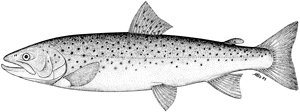
\includegraphics[width=.15\textwidth]{salmo_trutta_trutta.jpg}
      \end{turn}
      };
  \node[inner sep=0pt] (status) at (100pt,18pt)
      {
      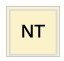
\includegraphics[width=0.5cm]{NT.jpg}
      };        
  \end{tikzpicture}
}%

\fbox{\begin{minipage}[t]{0.45\textwidth}
\par\small
\textcolor{bleu_EV}{
\titlefont{
La truite de mer \textit{Salmo trutta trutta} est un poisson migrateur
amphihalin qui se reproduit souvent plusieurs fois.
La reproduction a lieu en eau douce en novembre-janvier, avec un homing assez fort.
Environ 1/4 des truites de mer, majoritairement des mâles, seront sédentaires, 
les autres, majoritairement des femelles, dévaleront après 1 à 2 ans de vie en eau douce. 
Le séjour marin s'effectue à proximité des côtes françaises, avec des incursions fréquentes en eau douce. 
La durée de la phase marine est très variable, de quelques mois à 3 ans.
Les adultes de cette espèce peuvent rester en rivière, aller grossir en mer ou grossir 
en lac selon les contextes, ce qui définit trois écotypes distincts (truite fario, truite de mer et truite 
lacustre). La truite est classée en statut quasi menacé (NT) en France sur la
liste rouge UICN, il n'y a pas de classement pour les truites de mer mais elles sont
peu présente en Bretagne.
Sur la Vilaine, des alevinages de truites ont provoqué le passage d'environ 400 truites de mer en 1996,
puis les effectifs ont chuté très rapidement, pour être anecdotiques ces dernières années.
}}
\end{minipage}}
\smallskip

%vvv$TRM$N[vvv$TRM$N$annee==CY,"effectif"] 
Deux truites de mer dévalantes ont été %ont été
comptées en 2023 (Figure \ref{barplot_report_annual_trm}) %,  Tableau
%\ref{table_trm_mois}).
\begin{figure}[htpb]
\centering
\includegraphics[width=0.45\textwidth]{2023/barplot_report_annual_trm.png} 
\caption{Histogramme des effectifs annuels de truites de mer comptabilisés
au barrage d'Arzal.}
\label{barplot_report_annual_trm}
\end{figure}
%
%La migration est faible par rapport aux années précédentes (Figure
%\ref{table_bilanannuel_trm}, Tableau \ref{barchart_bmi_trm}).

%\begin{figure}[htpb]
%\centering
%\includegraphics[width=0.45\textwidth]{2023/barchart_bmi_trm.png} 
%\caption{Comparaison de la migration de truite de mer de CY avec la
%série interannuelle de données 1996-CY-1.}
%\label{barchart_bmi_trm}
%\end{figure}

%\input{vvv[["TRM"]][["path_y"]]} 

\input{C:/workspace/passe_bassins/table/2023/5_2224_IND_1996to2023.tex} 

La migration des truites de mer intervient toute l'année avec un pic estival
(Figure \ref{rmi_density_trm}). 
% En CY, la migration s'est faite en juin,
% juillet août et octobre Figures (\ref{barchart_bmi_trm},
% \ref{rmi_density_trm}).

\begin{figure}[htpb]
\centering
\includegraphics[width=0.45\textwidth]{2023/rmi_density_trm.png} 
\caption{Saisonnalité des migrations de truites de mer sur la Vilaine.}
\label{rmi_density_trm}
\end{figure}


Les tailles des truites mesurées au niveau de la passe d'Arzal sont présentées
en Figure \ref{size_trm}.

\begin{figure}[htpb]
\centering
\includegraphics[width=0.45\textwidth]{2023/size_trm.png} 
\caption{Taille des truites de mer mesurées au niveau du dispositif de
vidéocontrôle d'Arzal.}
\label{size_trm}
\end{figure}

%%%%%%%%%%%%%%%%%%%%%%%%%%%%%%%%%%%%%%%%%%%%%%%%%%%%%%%%%%%%%%%%%%%%%







\clearpage
\subsection{Autre espèces}


Par sa situation avec le pied en eau salée et la tête en eau douce, la passe ne
rencontre que des effectifs très faibles d'autres espèces. En 2023, les
espèces recensées sont assez
nombreuses, silure, sandre, black bass, cyprinidés et brème (Figure
\ref{autres_especes}). 
La fréquentation des autres espèces depuis 2000 est illustrée de manière
graphique à la Figure \ref{autres_especes_2000_2023}. 

\begin{figure}[htpb]
\centering
\includegraphics[width=0.45\textwidth]{2023/autres_especes.png} 
\caption{Effectif des autres espèces recensées en 2023 dans la passe,
\textit{Abramis brama} brème, 
\textit{Ameiurus melas} poisson-chat,
\textit{Sander lucioperca} sandre,
\textit{Cyprinus} carpe (genre), \textit{Cyprinidae} cyprinidés sans détermination,
\textit{Dichentrarchus labrax} bar commun,
\textit{Esox lucius} brochet,
\textit{Lampetra fluviatilis} lamproie fluviatile,
\textit{Perca fluviatilis} perche commune,
\textit{Rutilus rutilus} gardon,
\textit{Salmo trutta fario} truite fario,
\textit{Micropterus salmoides} black bass à grande bouche, 
\textit{Silurus glanis} silure,
\texit{Tinca tinca} tanche.}
\label{autres_especes}
\end{figure}



\begin{figure}[htpb]
\centering
\includegraphics[width=0.45\textwidth]{2023/autres_especes_2000_2023.png} 
\caption{Effectif des autres espèces rencontrées dans la passe d'Arzal depuis
2000.}
\label{autres_especes_2000_2023}
\end{figure}


\begin{figure}[htpb]
\centering
\includegraphics[width=0.45\textwidth]{2023/bilan_annuel_sil.png} 
\caption{Effectif des silures ayant migré par la passe d'Arzal depuis
2000.}
\label{bilan_annuel_sil}
\end{figure}


Les effectifs de silures recensés au niveau de la passe d'Arzal sont en très
nette augmentation (Figure \ref{bilan_annuel_sil}). De même, la tendances des
tailles mesurées est à l'augmentation, même si pour l'année 2023 les silures
étaient plus petits que les années précédentes (Figure \ref{size_sil}).

\begin{figure}[htpb]
\centering
\includegraphics[width=0.45\textwidth]{2023/size_sil.png} 
\caption{Taille des silures mesurés au niveau du dispositif de vidéocontrôle
d'Arzal.}
\label{size_sil}
\end{figure}


\input{C:/workspace/passe_bassins/table/2023/5_2238__1996to2023.tex} % table bilan silures



















\clearpage
\onecolumn
\section{Annexes}

Pour l'étude glanispomi, il est nécessaire de calculer la biomasse de poissons
migrant sur la Vilaine pour les mois de mars à mai pour les aloses, lamproies et
mulets. L'objectif est de faire ce calcul pour 2023 mais aussi pour les années
précédentes.




\paragraph{Calculs extraits de la base de données du barrage.}

La base de données du barrage collecte les informations relatives aux niveaux et
au fonctionnement des vannes au pas de temps de 10 minutes. Le fichier des données extrait de la base de données du barrage
contient \textcolor{orange_EV}{\num{50622}} lignes. A partir de ce dernier,
un script de traitement extrait les temps et les modes de fonctionnement de la
passe (Figure \ref{figure_schema_fonctionnement}). 
Les sondes utilisées en
référence ont parfois des valeurs manquantes,
 \textcolor{orange_EV}{\num{0}} et \textcolor{orange_EV}{\num{2}} respectivement 
 pour les niveaux aval (mer) et amont (Vilaine).
Pour les niveaux mer, après correction, en utilisant l'une ou l'autre des
sondes, le nombre de valeurs manquantes restantes pour lesquelles les deux sondes n'ont pas de
valeur est de \textcolor{orange_EV}{\num{37}}. En Vilaine
cette année, la correction correspond à
\textcolor{orange_EV}{\num{37}} lignes pour les
niveaux aval et amont.
Les corrections des niveaux de la mer\footnote{Suppression
des valeurs inférieures à -3.5 m NGF.} correspondent à
\textcolor{orange_EV}{\num{0}} lignes, celles du sas aval \footnote{Le dernier
bassin en aval de la passe, la différence de niveaux entre ce bassin et la mer conditionne le
fonctionnement de la vanne aval, suppression des valeurs en dehors de la gamme
[-1m,2.5m].} correspondent à \textcolor{orange_EV}{\num{1398}} lignes et des
dérives de codeur sur la vanne mer \footnote{Suppression des valeurs en dehors de la gamme
[-1.72m,2.5m] correspondant à la course normale de la vanne.} à
\textcolor{orange_EV}{\num{0}} lignes. 
Au final \textcolor{orange_EV}{\num{204}} lignes manquent des données permettant de
calculer le fonctionnement de la passe (Figure \ref{figure_fonctionnement_passe}). Le fichier de calcul des temps de
fonctionnement réintégré dans stacomiR comporte
\textcolor{orange_EV}{\num{2824}} lignes.
\begin{figure}[htpb]
\centering
\includegraphics[width=\textwidth]{2023/detail_fonct_passe_2.png}
\caption{Illustration du fonctionnement de la passe lors d'un fonctionnement
normal en mai. A chaque cycle de marée, le niveau de la mer varie entre +2 m et
-2m environ (en noir). Le niveau Vilaine (.- bleu) varie peu et reste
autour de 1m80. La vanne amont (en marron clair) s'ouvre  dès que le niveau mer
descend 30 cm en dessous du niveau Vilaine, c'est l'entrée en régulation de la
passe. La vanne aval (.... violets) ajuste le niveau du SAS (courbe bleue)
pour maintenir une chute constante à l'aval de la passe à l'aide d'une
régulation par l'automate. 
 L'arrêt pour maintenance le 17 lors de la marée montante se traduit par une
 fermeture de la vanne amont (trait horizontal supplémentaire). L'état de la
 passe est calculée pour chaque période de 10 minutes (en bas).
}
\label{detail_fonct_passe_2}
\end{figure}


\begin{figure}[htpb]
\centering
\includegraphics[width=0.8\textwidth]{2023/detail_fonct_passe_1.png}
\caption{Illustration du fonctionnement de la passe après la remise en route
de la passe en avril. En ordonnée, les niveaux mer (noir), vilaine
(.-), sas (en bleu), niveau vanne mer (pointillés violet), niveau vanne Vilaine (ligne marron
continue). L'état de la passe est calculée pour chaque période de 10 minutes (en bas).
Les 10 et 11 après midi, la position basse de la vanne amont (vanne fermée)
indique une fermeture de la passe.}
\label{detail_fonct_passe_1}
\end{figure}


\begin{figure}[ht]
\centering
\includegraphics[width=0.6\textwidth]{2023/debit_passe_mesure.png}
\caption{Débit calculé dans la passe en 2023, mesures de l'automate du barrage.}
\label{debit_passe_mesure}
\end{figure}


\begin{figure}[ht]
\centering
\includegraphics[width=0.6\textwidth]{2023/debit_passe_calcul.png}
\caption{Débit recalculé dans la passe en 2023, après correction des valeurs
aberrantes et prise en compte du noyage aval de la passe.}
\label{debit_passe_calcul}
\end{figure}


\begin{figure}[hp]
\centering
\includegraphics[width=0.9\textwidth]{2023/report_df_annee.png} 
\caption{Bilan du fonctionnement de la passe lors de l'année 2023. En orange
il est possible de suivre les périodes de haute mer où la passe est fermée, les
périodes où les bandes sont les plus larges correspondent à des périodes de
vives eaux et également en hiver aux périodes où la gestion de la
Vilaine est plus réduite. Les arrêts nocturnes de la passe sont visibles en mai
- juin - juillet. En septembre et octobre, le passage en "mode étiage" réduit la
durée de fonctionnement de la passe aux quelques heures qui précèdent la marée
haute. En hiver, en période de crue, la passe est à l'arrêt.}
\label{report_df_annee}
\end{figure}

%\begin{figure}[hp]
%\centering
%\includegraphics[width=0.95\textwidth]{2023/report_df_fct_2003_2010.png} 
%\caption{Bilan mensuel du fonctionnement de la passe à bassins d'Arzal de 2003
%à 2010.}
%\label{report_df_fct_2003_2010}
%\end{figure}




\begin{figure}[hp]
\centering
\includegraphics[width=\textwidth]{2023/bmm_alose.png}
\caption{Bilan de la migration des aloses en 2023. Effectifs journaliers et
fonctionnement des dispositifs de franchissement et de comptage.}
\label{bmm_alose}
\end{figure}

\begin{figure}[hp]
\centering
\includegraphics[width=\textwidth]{2023/bmm_mulet.png}
\caption{Bilan de la migration des mulets en 2023. Effectifs journaliers et
fonctionnement des dispositifs de franchissement et de comptage.}
\label{bmm_mulet}
\end{figure}


\begin{figure}[hp]
\centering
\includegraphics[width=\textwidth]{2023/bmm_lpm.png}
\caption{Bilan de la migration des lamproies marines en 2023. Effectifs
journaliers et fonctionnement des dispositifs de franchissement et de comptage.}
\label{bmm_lpm}
\end{figure}




\paragraph{Entretien de la passe}
L'historique des modifications effectuées depuis la mise en service de
la passe à bassins est décrit au Tableau \ref{table_entretien_passe}.

\begin{table}[htb]
\begin{tabular}{p{0.1\textwidth}p{0.8\textwidth}}
\toprule
Année & Intervention\\
\midrule
1998 & Mise en place du mode "étiage" pour maintenir le fonctionnement
de la passe à bas débit.\\
2000 & Reprogrammation des automatismes pour éviter le vieillissement
prématuré de la centrale hydraulique aval.\\
2005 & Changement du système vidéo, remplacement par un système
numérique. \\
2005 & Changement de la vanne aval (corrosion).\\
2010 &  Remplacement des têtes des vérins aval corrodées par des têtes en
inox.\\
2011 & Modernisation des armoires électrique amont et aval,
reprogrammation des automatismes.\\
2012 & Pose d'une vanne montée sur poulie sur le canal de débit d'appoint
pour faciliter la réouverture rapide du canal, et favoriser la gestion
d'étiage.\\
2013 & Rénovation du local d'accueil de la passe à bassins (peinture,
gradin).\\
2014 & Rénovation du local d'accueil de la passe à bassins (téléviseur,
luminaires, prises \ldots{}).\\
2016 & Réparation du caisson lumineux après plusieurs submersions. Etude
de la possibilité d'installer un caisson étanche avec un éclairage par
leds.\\
2017-18 & Rénovation des vérins de la porte aval.\\
2020 & Changement de pièces sur les vérins de la porte aval.\\
2021 & Renforcement des structure du capteur de fin de course aval, Remplacement
des joints de la vanne intermédiaire.\\
2022 & Aucune modification particulière effectuée\\
2023 & Remplacement des néons led du caisson lumineux. Changement de la sonde de niveau du SAS. Installation d’un chauffage et d’un déshumidifacteur afin de préserver de matériel électronique
de la passe à bassin. Changement des boîtiers électroniques des sondes de
niveaux amont et aval du barrage.\\
\bottomrule
\end{tabular}
\caption{Entretien historique de la passe à bassins.}
\label{table_entretien_passe}
\end{table}





\clearpage
Versions précédentes des rapports annuels (table \ref{table_references}).


\begin{table}[htbp]
\centering
\caption{Rapports précédents concernant la passe à bassins.}
\begin{tabular}{lp{7cm}}
\toprule
Année & Rapport \\
\midrule
2023 &
\href{https://eptbvilaine56.sharepoint.com/:b:/g/extranet/EUqlfhsKgqpMkzWSuEo9uRABXEw73VtgoVhM8t-C6zGTiQ?e=MuQwCG}{Suivi
de la passe à bassins, 2022} \\
2022 &
\href{https://eptbvilaine56.sharepoint.com/:b:/g/extranet/EabAMF4YvrJJhxYU8-pm6JwBSLrjt05hvlhTO2kxb84Aag?e=yvfCUS}{Suivi
de la passe à bassins, 2021} \\
2021 &
\href{https://eptbvilaine56.sharepoint.com/:b:/g/extranet/EX0SnyoGmBlMsO-6-Il8wugBCHYxha3l2A-5tA9yTCqwbg?e=XukC2d}{Suivi
de la passe à bassins, 2020} \\
2020 &
\href{https://eptbvilaine56.sharepoint.com/:b:/g/extranet/EQl4smhm635FgMPzE9bFyxsB_9ZMmVLH34BJLfwieJKuUA?e=dtqKYE}{Suivi
de la passe à bassins, 2019} \\
2019 &
\href{https://eptbvilaine56.sharepoint.com/:b:/g/extranet/ESlFdwgrzNZPjHy2CamDrh4Bd-wJB1BhJ-Hf19RuTZlpgw?e=3pPkHa}{Dynamique de la population de Mulet porc \textit{Chelon ramada} (Risso 1827) dans le bassin versant de la Vilaine}\\
2019 & 
\href{https://eptbvilaine56.sharepoint.com/:b:/g/extranet/EfsNAFGO4sRAoEb-9-SEERoBJAxYBJVWvF-9OVVryuF8QA?e=G5x6Ij}{Suivi
de la passe à bassins, 2018}\\
2018 &
\href{https://eptbvilaine56.sharepoint.com/:b:/g/extranet/EddDt8hE-z5KvA3qWm8RiUYBiawsguFwtT101pmeEXjEiQ?e=TdLuRC}{Suivi
de la passe à bassins, 2017}\\
2017 &
\href{https://eptbvilaine56.sharepoint.com/:b:/g/extranet/EZovsRks3WFKsse_rsnnqh0BAcwjBH5ofFK1pjdwtAe6Dw?e=sRP0k9}{Suivi
de la passe à bassins, 2016}\\
2016 &
\href{https://eptbvilaine56.sharepoint.com/:b:/g/extranet/EUaIB9CdQItLkPTR0banFZYBv7DnfD7uNSezUSFVD9tfcw?e=ZAWC9t}{Suivi
de la passe à bassins, 2015}\\
2015 &
\href{https://eptbvilaine56.sharepoint.com/:b:/g/extranet/EQCdJUAzgLlJpqe-HgXcbn4BvTlV7Xool5zCmmV-fZaolg?e=dvEObL}{Suivi
de la passe à bassins, 2014}\\
2014 &
\href{https://eptbvilaine56.sharepoint.com/:b:/g/extranet/Effnw5jtEPFHmxCcqlWiTBsB0Cm29yADN5bSREbOi1yTzA?e=YS1Ref}{Suivi
de la passe à bassins, 2013}\\
2013 &
\href{https://eptbvilaine56.sharepoint.com/:b:/g/extranet/Ed6J-KFKTc1EhcXyxox1eU4B86i9IYhY53FuP2ilW9TdhA?e=pagXSD}{Suivi
de la passe à bassins, 2012}\\
2012 &
\href{https://eptbvilaine56.sharepoint.com/:b:/g/extranet/EWQJkGynJO9FkLtMc0evglwBhVC3k2ORqwqhA_ez-fecKQ?e=xaK6zo}{Suivi
de la passe à bassins, 2011}\\
2010 &
\href{https://eptbvilaine56.sharepoint.com/:b:/g/extranet/ETTqqTILtm5OjioHyGGAsooBsGVP5CgR9fE-xCj-evifLA?e=2I4CbN}{Suivi
de la passe à bassins, 2009}\\
2009 &
\href{https://eptbvilaine56.sharepoint.com/:b:/g/extranet/ESOYjucqRlRNm4hXNuO3-EgBBOTq0zMqmhq0u125J21Yxw?e=EbCzao}{Suivi
de la passe à bassins, 2008}\\
%
\bottomrule
\end{tabular}
\label{table_references}
\end{table}

\bigskip
\paragraph{Remerciements}

La passe fonctionne au quotidien grâce au travail d'entretien, de suivi et
d'intervention des barragistes : Alban Le Guen, Cyril Faucon, Johann Dahlem,
Laurent Philippot, Thierry Besnard. Nous tenons à les remercier pour leur aide
et leur disponibilité.
\bigskip

\vfill
\paragraph{Ressources en ligne} ~

Observatoire des poissons migrateurs en Bretagne~:
\href{http://www.observatoire-poissons-migrateurs-bretagne.fr}{{http://www.observatoire-poissons-migrateurs-bretagne.fr}}

Association Loire Grands Migrateurs (LOGRAMI)~:
\href{http://www.logrami.fr}{{http://www.logrami.fr}}

Migrateurs Garonne Dordogne Charente Seudre (MIGADO)~:
\href{http://www.migado.fr}{{http://www.migado.fr}}

Cellule Migrateurs Charente Seudre (MIGADO)~:
\href{http://www.migrateurs-charenteseudre.fr}{{http://www.migrateurs-charenteseudre.fr}}

Saumon-Rhin~:   
\href{https://www.saumon-rhin.com/}{{https://www.saumon-rhin.com/}}

Fédération de pêche de la Somme ~: 
\href{https://peche80.com/}{{https://peche80.com/}}

Seine-Normandie Migrateurs (SEINORMIG)~:    
\href{https://www.seinormigr.fr/}{{https://www.seinormigr.fr/}}

Stations de suivi INRAe-OFB~:      
\href{https://bretagne-environnement.fr/bresle---oir---scorff---nivelle-trois-decennies-observations-recherche-poissons-migrateurs}{{https://bretagne-environnement.fr/bresle---oir---scorff---nivelle-trois-decennies-observations-recherche-poissons-migrateurs}}

Migrateurs Adour (MIGRADOUR)~:                          
\href{https://www.migradour.com/activite/site-index-soustons/}{{https://www.migradour.com/activite/site-index-soustons/}}

Migrateurs Rhône-Méditerranée (MRM)~:            
\href{https://www.migrateursrhonemediterranee.org/}{{https://www.migrateursrhonemediterranee.org/}}



%\twocolumn
% biblio commune aux différentes années
\printbibliography

\clearpage

\onecolumn
\thispagestyle{empty}
\pagecolor{bleu_EV}
\begin{tcolorbox}[enhanced jigsaw,
                  colback=turquoise_EV!30,%gray background
                  colframe=turquoise_EV,% black frame colour
                  width=\textwidth,% Use 5cm total width,
                  arc=3mm, auto outer arc,
                  boxrule=5pt,
                  drop shadow={bleu_EV!50!gray!80}
                 ]
\textbf{Résumé}\par

 \vspace{8mm}
    
 Ce rapport présente le bilan de suivi de la passe à bassins d'Arzal en
    \textcolor{orange_EV}{\num{2023}}. Il détaille le fonctionnement de la passe, de son système
    d'enregistrement vidéo, ainsi que les effectifs annuels des principales
    espèces ayant transité par la passe du barrage d'Arzal à l'estuaire de la
    Vilaine. En \textcolor{orange_EV}{\num{2023}}, 
    \textcolor{orange_EV}{\num{538}} aloses (\textit{Alosa
    Sp.}), 
    \textcolor{orange_EV}{\num{1150}} lamproies marines (\textit{Petromyzon
    marinus}), 
    \textcolor{orange_EV}{\num{-2}} truites de mer (\textit{Salmo trutta trutta}),
    \textcolor{orange_EV}{\num{16}} saumons (\textit{Salmo salar}) et
    \textcolor{orange_EV}{\num{102972}} mulets porcs (\textit{Chelon ramada}) ont été
    comptabilisés à la passe d'Arzal.  \par
        
   \vspace{8mm}
    
   \textbf{Abstract}\par
   
    \vspace{8mm}
  
    This report presents the monitoring of the pool fishway at Arzal in
    \textcolor{orange_EV}{\num{2023}}. It details the operation of the fishway and it's recording video
    device, along with the annual number of the main species crossing the Arzal
    Dam in the Vilaine esturay.
    In \textcolor{orange_EV}{\num{2023}}, 
    \textcolor{orange_EV}{\num{538}} shads (\textit{Alosa Sp.}),
    \textcolor{orange_EV}{\num{1150}} sea lampreys (\textit{Petromyzon marinus}), 
    \textcolor{orange_EV}{\num{-2}} sea trouts (\textit{Salmo trutta trutta}),
    \textcolor{orange_EV}{\num{16}} salmons (\textit{Salmo salar}) 
    and \textcolor{orange_EV}{\num{102972}} mulets (\textit{Chelon ramada}) have been
    counted at the Arzal fishway. \par

   

    \vspace{8mm}
    \textbf{Mots clés:}\par
     \textit{mulet, lamproie marine, alose, stacomi}\par 
    \vspace{8mm}    
     \textbf{\textit{Keywords:}}\par
     \textit{mulet, lamprey, shad, stacomi}  
\end{tcolorbox}


\vfill
\color{turquoise_EV}
\hfill\makebox[0.5\textwidth][r]{%
\begin{minipage}{0.4\textwidth}  
\tiny
\noindent\hrulefill\par 
\noindent Rapport \LaTeX \par
packages R : \vspace{1mm}

StacomiR \colcitep{turquoise_EV}{briand_stacomir_2017}\par
\LaTeX \ :Hmisc, xtable, stargazer, tables, knitr \par
graphiques : stacomiR, ggplot2, lattice, ggthemr, packcircles, colorspace\par
traitements : stringr, lubridate, reshape2, dplyr\par
diagrammes : diagrammeR \\
base : readxl, RPostgres, DBI, stacomirtools\par
\vspace{1mm}
Dernière compilation : le \today\par
R version 4.2.3 (2023-03-15 ucrt)\par
\noindent\hrulefill\par
\end{minipage}}

\clearpage

\end{document}

